% =====================================================================
%  ISDS 2026 -- The 4th International Conference on Intelligent Systems
%  and Data Science, Yuan Ze University, Taiwan, 14-15 November 2026
%
%  Submission format required by the conference:
%    * Springer LNCS/CCIS ONE-COLUMN page format (llncs.cls)
%    * Long paper: 12-15 pages   /   Short paper: 6-8 pages
%    * English, PDF, submitted via EasyChair (conf=isds2026)
%    * LaTeX template preferred over Word
%  Reference: https://isds.ctu.edu.vn/2026/  and
%  https://www.springer.com/gp/computer-science/lncs/conference-proceedings-guidelines
%
%  Track: Track 3 -- Image Processing & Pattern Recognition
%  Build:  pdflatex ISDS2026_FGSS  (x2)
% =====================================================================
\documentclass[runningheads]{llncs}

\usepackage{cmap}
\usepackage[T1]{fontenc}
\usepackage[utf8]{inputenc}
\usepackage{amsmath,amssymb,amsfonts}
\usepackage{graphicx}
\usepackage{textcomp}
\usepackage[table]{xcolor}
\usepackage{booktabs}
\usepackage{multirow}
\usepackage{array}
\usepackage{url}
\usepackage{float}
\usepackage{placeins}
\usepackage{colortbl}
\usepackage{tcolorbox}
\tcbuselibrary{skins}
\usepackage{algorithm}
\usepackage{algpseudocode}

% hyperref last; Springer prefers non-coloured links in the final PDF
\usepackage[hidelinks]{hyperref}

% \doi is provided by recent llncs.cls / splncs04.bst; define it if missing
\providecommand{\doi}[1]{\href{https://doi.org/#1}{https://doi.org/#1}}

% ---- palette retained from the drawio-flavoured figures (mono-print safe) ----
\definecolor{drawioBlueLine}{HTML}{6C8EBF}
\definecolor{drawioOrangeLine}{HTML}{D79B00}
\definecolor{drawioGreenLine}{HTML}{82B366}
\definecolor{drawioPurpleLine}{HTML}{9673A6}

% ---- readability: table spacing + reusable "takeaway" box ----
\renewcommand{\arraystretch}{1.15}
\setlength{\tabcolsep}{4pt}
\definecolor{takeawayline}{HTML}{6C8EBF}
\definecolor{takeawayfill}{HTML}{EEF4FC}
\definecolor{rowshade}{HTML}{F2F2F2}
\newtcolorbox{takeaway}{
  colback=takeawayfill, colframe=takeawayline, boxrule=0.6pt,
  arc=2pt, left=6pt, right=6pt, top=4pt, bottom=4pt,
  fontupper=\small
}

\renewcommand{\topfraction}{0.85}
\renewcommand{\bottomfraction}{0.70}
\renewcommand{\dbltopfraction}{0.85}
\renewcommand{\textfraction}{0.10}
\renewcommand{\floatpagefraction}{0.75}
\renewcommand{\dblfloatpagefraction}{0.75}

\begin{document}

\title{Frequency-Guided Semantic Steganography for High-Fidelity Self-Contained Style-Transfer Image Hiding}

\titlerunning{Frequency-Guided Semantic Steganography}

\author{%
Ngoc-Giau Pham\inst{1,2} \and
Phu-Thanh Ha-Quach\inst{3} \and
Hong-Ngoc Tran\inst{3}\textsuperscript{(\textrm{*})}%
}

\authorrunning{N.-G. Pham, P.-T. Ha-Quach, and H.-N. Tran}

\institute{%
School of Engineering and Technology, Tra Vinh University, Vinh Long, Vietnam
\and
Faculty of Engineering and Technology, Tien Giang University, Dong Thap, Vietnam\\
\email{phamngocgiau@tgu.edu.vn}
\and
Faculty of Engineering, Vietnamese-German University, Ho Chi Minh City, Vietnam\\
\email{thanhbo025@gmail.com}, \email{ngoc.th@vgu.edu.vn}\\[2pt]
\textsuperscript{(\textrm{*})}\,Corresponding author: Hong-Ngoc Tran (\email{ngoc.th@vgu.edu.vn})
}

\maketitle

\begin{abstract}
% SOURCE: run_summary.json, paper_table_main.csv, token_summary.csv, ablation.csv, robustness_metrics.csv, metrics.json
Style-transfer steganography uses artistic brushstrokes to mask data-hiding perturbations, yet existing methods rarely exceed $38$\,dB cover PSNR and remain brittle under serial re-stylisation. We trace this limitation to two implicit design choices: an unbounded capacity penalty that leaks embedding energy into low-frequency structure, and a spatial payload representation that is expensive for the carrier to absorb. We address both with a frequency-guided semantic steganography network (FGSS). The secret is compressed into a compact $32\!\times\!32\!\times\!64$ semantic token plus a thumbnail, reducing payload bandwidth by approximately three-fold relative to the full-resolution secret. A non-linear \emph{capacity-ceiling} penalty maps a target PSNR to a soft barrier on cover MSE, and a discrete-wavelet-inspired \emph{frequency loss} confines the residual to the high-frequency band. An oracle-distilled reverse decoder and a probabilistic serial-future pass enable self-contained stylisation that survives up to three re-stylisations. On $600$ evaluation pairs drawn from COCO\,val2017 with five painting styles, the model achieves $39.61\pm0.35$\,dB cover PSNR, $0.9914$ SSIM, and lifts reverse SSIM from $0.52$ (naive) to $0.81$ (token-conditioned), while token MSE drifts by less than $1\!\times\!10^{-4}$ under JPEG and Gaussian attacks. A controlled ablation shows the ceiling alone contributes $+5.76$\,dB. Cross-dataset evaluation on four unseen benchmarks (DIV2K, CelebA, BOSSBase, COCO) confirms $\approx\!40$\,dB PSNR stability, and a robustness audit across $11$ attack types confirms that token-MSE deviations remain below $0.002$ under standard image-processing attacks. Furthermore, these deviations stay below $0.012$ even after serial re-stylisation. The system trains in approximately $10$ hours on a single A100 GPU and runs end-to-end on a CPU ($228$\,k parameters).

\keywords{Image steganography \and Neural style transfer \and Frequency-domain learning \and Capacity ceiling \and Robustness \and Semantic tokens \and Self-contained stylisation.}
\end{abstract}

\section{Introduction}

Hiding information inside ordinary-looking images has been a fundamental technique in digital communication for several decades. Deep learning has substantially extended the achievable payload capacity relative to LSB-based predecessors; however, this additional capacity is not without cost. The residuals introduced by deep encoders exhibit statistical fingerprints that contemporary steganalysers detect with considerable accuracy~\cite{isn,riis,rmsteg}. One countermeasure is to alter the statistical properties of the carrier itself: when the cover is a painting rather than a photograph, brush strokes and palette quantisation already introduce a degree of noise within which small additive perturbations remain visually plausible. This observation motivates \emph{style-transfer steganography}~\cite{wacv2020,stylestegan2023,sstegogan2024,sst2024,ihst2024,css2024,sddpm2025,stisgan2026}, and in particular its most demanding variant, \emph{self-contained} stylisation~\cite{wacv2020}, in which the stego image alone must carry sufficient information for the receiver to reconstruct the original content by inverting the stylisation process.

In practice, however, the design space of style-transfer steganography is constrained by an unfavourable coupling between its two objectives. Increasing the embedding strength improves secret recoverability but introduces visible texture jitter and palette drift; reducing it preserves the cover but degrades reverse extraction. Even when the cover is well preserved, applying a second or third style transfer to the stego image --- \emph{serial} stylisation --- typically destroys most of the embedded information~\cite{wacv2020,stylestegan2023}. Consequently, most reported systems occupy a narrow region of this trade-off space, with cover PSNR seldom exceeding $35$\,dB, reverse SSIM below $0.6$, and serial recovery degrading rapidly beyond the second stylisation step.

\begin{figure}[!t]
\centering
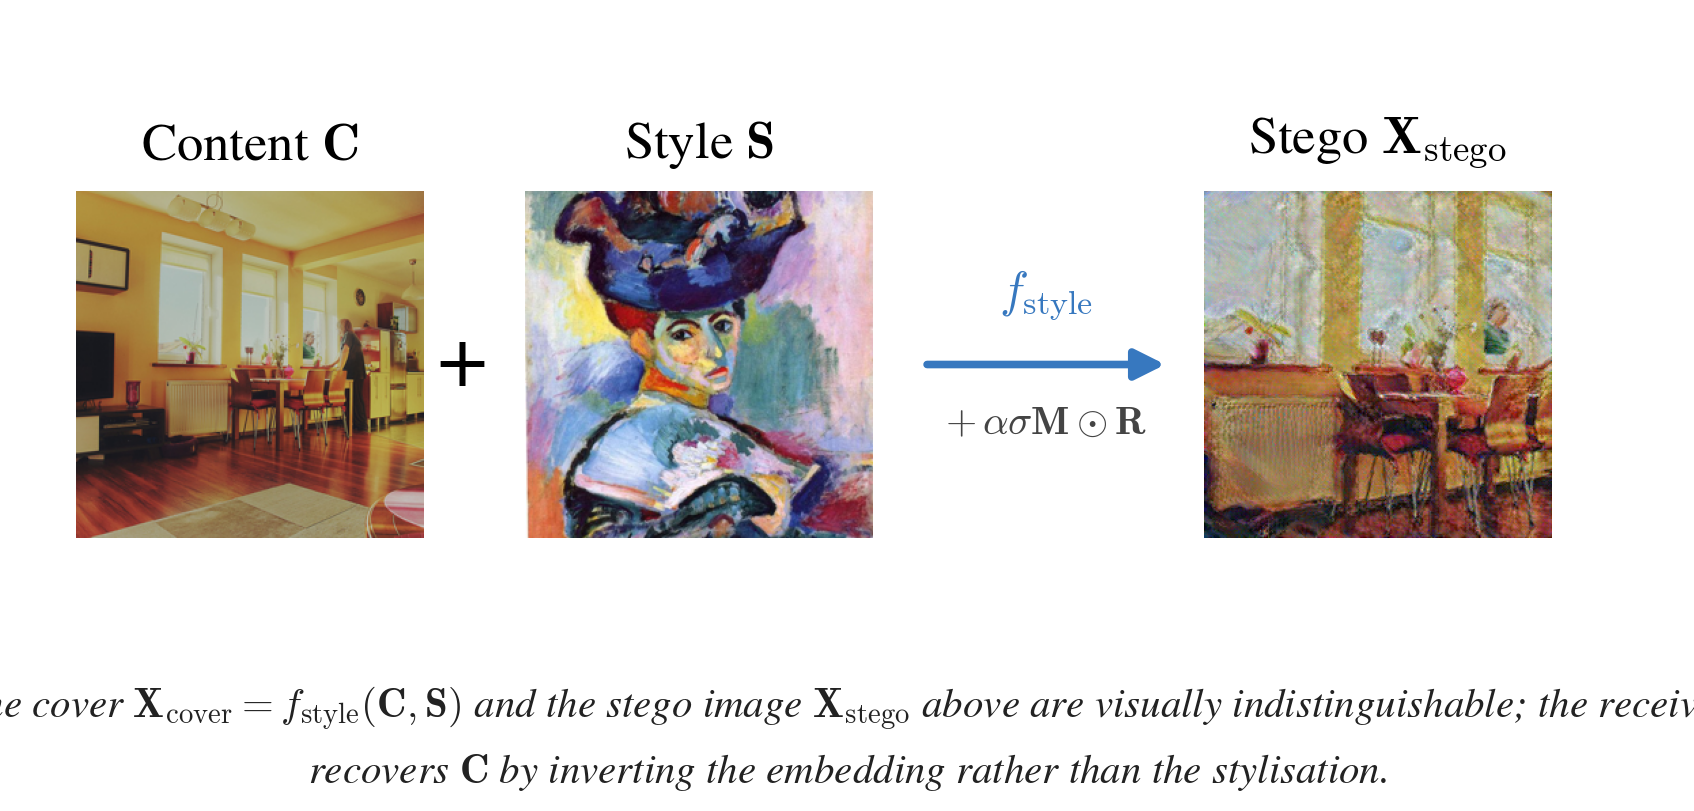
\includegraphics[width=0.86\textwidth]{paper_assets/intro_teaser.png}
\caption{Concrete illustration of self-contained stylisation. The content and style images are combined by the cover generator $f_{\text{style}}$ to produce a stylised cover, into which FGSS embeds a bounded residual to obtain the stego image shown. The example uses real images from the evaluation set; quantitative fidelity is reported in Table~\ref{tab:cover}.}
\label{fig:introteaser}
\end{figure}

Figure~\ref{fig:introteaser} illustrates this concept concretely using an example from the evaluation set: the stego image on the right is produced by embedding a payload into the stylised cover, and is visually indistinguishable from it.

We attribute this limitation to two design choices that are typically made implicitly rather than deliberately in published methods. The first is an \emph{unbounded payload-capacity loss}: the encoder is encouraged to keep the residual small only through a quadratic prior, which imposes no upper bound. Once the optimiser identifies a configuration that decodes successfully, nothing prevents it from placing that solution in the low-frequency, structurally salient component of the carrier, to which the human visual system is most sensitive. The second is a \emph{spatial payload representation}: secret images, dense bit grids, and even feature maps occupy approximately as many spatial positions as the cover itself, which forces the encoder to distribute its perturbation broadly and leaves little capacity for the carrier to absorb a subsequent stylisation pass.

This paper addresses both limitations directly. In place of the spatial payload, the secret is distilled into a compact semantic token $\mathbf{z}\!\in\!\mathbb{R}^{64\times32\times32}$ together with a low-resolution thumbnail $\mathbf{T}$, both produced by a small CNN tokenizer. In place of the unbounded prior, the residual is bounded using a non-linear \emph{capacity-ceiling} window: a quadratic penalty that activates only above an explicit threshold $\epsilon$ tied directly to a target cover PSNR. A \emph{frequency-guided} loss, inspired by the discrete wavelet decomposition, further constrains the spectral allocation of the residual: it decomposes the residual into low- and high-frequency bands via a strided average-pooling operator and its bilinear up-sampler, penalises the low band aggressively, and leaves the high band unconstrained, thereby directing the perturbation into texture rather than into the structural components most salient to the human visual system. Three additional mechanisms complete the system: an \emph{oracle-distilled} reverse loss, a \emph{serial-source} consistency term that remains effective after one or two additional re-stylisations, and a band-by-band \emph{embedding-allocation} loss that further constrains where the encoder may place its energy.

% SOURCE: run_summary.json (cover_metrics_mean), token_summary.csv, ablation.csv
This combination requires modest computational overhead --- $228\,435$ learnable parameters across all three modules at $192\!\times\!192$ --- while yielding substantial empirical improvements. On the COCO~val2017~\cite{coco} evaluation protocol with $600$ content--style pairs and five painting-style references, the model achieves a cover PSNR of $39.61\pm0.35$\,dB, an SSIM~\cite{ssim} of $0.9914\pm0.0030$, and an LPIPS~\cite{lpips} of $0.0195\pm0.0081$, while the token MSE varies by less than $1\times10^{-4}$ under JPEG-style smoothing and additive Gaussian perturbations. A controlled CPU-only ablation attributes this improvement primarily to the capacity ceiling, which alone accounts for a $+5.76$\,dB increase in cover PSNR ($35.61\to41.37$\,dB); the frequency loss preserves this fidelity while leaving extraction performance unaffected. The contributions of this paper are summarised as follows:
\begin{itemize}
    \item A \emph{capacity-ceiling} formulation that explicitly maps a target cover PSNR to a soft non-linear barrier on the cover MSE, removing the implicit trade-off between cover fidelity and extraction quality.
    \item A differentiable \emph{frequency-guided} loss that uses a strided average-pooling proxy of the discrete wavelet transform to constrain the residual to the high-frequency band, without introducing new learnable parameters, and a complementary band-localised \emph{embedding allocation} loss that pushes the embedding spectrum towards a target shape.
    \item A \emph{semantic-token} payload (a $32\!\times\!32\!\times\!64$ feature grid concatenated with a $32\!\times\!32$ RGB thumbnail) that compresses the secret into a low-bandwidth representation, allowing the carrier to absorb it under both the ceiling and the frequency constraints.
    \item An \emph{oracle-distilled} reverse extraction stack and a probabilistic \emph{serial-future} pass that together stabilise self-contained stylisation under one or two further re-stylisations of the cover.
    \item A controlled experimental study on COCO with $600$ evaluation pairs and five painting styles, including (i) a comparison against fifteen modern image-steganography methods, (ii) reverse and serial-step recovery tables under three attack channels (clean, JPEG-style, Gaussian), (iii) a CPU-side ablation that isolates the role of the ceiling and the frequency loss, and (iv) a CPU inference budget showing that the framework is deployable outside GPU clusters.
\end{itemize}

\section{Related Work}

\subsection{Deep Image-in-Image Steganography}
The first wave of deep steganography embedded one full-resolution image inside another, using encoder--decoder networks or generative adversarial models. ISN~\cite{isn} introduced an invertible neural network (INN) that achieves a favourable container/secret PSNR balance; RIIS~\cite{riis} subsequently incorporated robust flow blocks that tolerate moderate Gaussian noise and JPEG compression. RMSteg~\cite{rmsteg} replaced the secret image with a QR-coded message routed through an attention-flow stack, reporting strong bit-error-rate (BER) performance under print-photo channels, while Robust-Frequency-Stego~\cite{rfs2023} extended the design into the frequency domain, training an embedding network that minimises BER across a JPEG quality sweep. These methods perform well on photorealistic carriers, but this capability incurs a cost in distinguishability: even small perturbations shift a natural image's statistics in ways that SRNet~\cite{srnet}, XuNet~\cite{xunet}, and SRM-class~\cite{srm} steganalysers are specifically trained to detect.

\subsection{Coverless and Steganography-Without-Embedding}
A second family avoids the cover-modification problem entirely, either generating a stego image from scratch or mapping the secret onto an existing image without pixel-level modification. IDEAS~\cite{ideas2022} introduced a disentanglement autoencoder for steganography-without-embedding (SWE), demonstrating that pixel perturbation is unnecessary provided the receiver can execute the same decoder. SI-SWE~\cite{siswe2023} hardened this approach against tamper attacks, and CRoSS~\cite{cross} extended it further using a diffusion model that synthesises containers conditioned on semantic secrets. This family offers substantial immunity to traditional steganalysis, but at the cost of bandwidth: the payload is compressed aggressively, and the carrier offers limited control over its final appearance. The present work adopts the SWE intuition that secrets are best represented as semantic tokens, but couples this representation with a deterministic NST carrier and a residual that is bounded rather than zero.

\subsection{Style-Transfer Steganography}
The third family, which this work builds upon, deliberately uses an artistic style as a means of concealing the embedding noise. Self-contained stylisation~\cite{wacv2020} established the foundational approach, embedding an inverse-mapping representation within the stylised image so that the original photograph can subsequently be recovered. Quaternion-style stego~\cite{quat2021} performed the manipulation in the frequency domain via quaternion algebra; StyleStegan~\cite{stylestegan2023} embedded at the feature level instead. The field has since diversified considerably: Style-Stego-GAN~\cite{sstegogan2024}, Steganography-in-Style-Transfer~\cite{sst2024}, IHST~\cite{ihst2024}, Constructive-Style-Stego~\cite{css2024}, StyleTransfer-DDPM-Stego~\cite{sddpm2025}, and STIS-GAN~\cite{stisgan2026} each introduced progressively more elaborate architectures, including conditional transformers, geometric mappings, latent diffusion, and frequency-attention modules. Despite this architectural progress, an explicit and mathematically grounded barrier on cover distortion remains rare; most existing work instead relies on a single quadratic regulariser with a manually tuned coefficient. Section~\ref{sec:method} addresses this gap by introducing a capacity ceiling whose threshold is computed directly from the desired PSNR rather than determined empirically.

Table~\ref{tab:relwork} summarises the three families discussed above and indicates which aspects of each FGSS retains: a bounded, non-zero residual from the coverless family, the semantic-token intuition from the steganography-without-embedding literature, and the style-transfer carrier itself, extended with the capacity-ceiling barrier described in Section~\ref{sec:method}.

\begin{table}[t]
\centering
\caption{Positioning of FGSS relative to the three families of related work discussed in this section. FGSS is closest to the style-transfer family but incorporates design elements motivated by the other two.}
\label{tab:relwork}
\setlength{\tabcolsep}{4pt}
\footnotesize
\begin{tabular}{@{}p{0.20\textwidth}p{0.24\textwidth}p{0.26\textwidth}p{0.19\textwidth}@{}}
\toprule
\textbf{Family} & \textbf{Representative methods} & \textbf{Key trade-off} & \textbf{What FGSS retains} \\
\midrule
\textcolor{drawioPurpleLine}{\textbf{Deep Image-in-Image Steganography}} &
ISN~\cite{isn}, RIIS~\cite{riis}, Robust-Freq~\cite{rfs2023}, RMSteg~\cite{rmsteg} &
High capacity, but residuals are statistically detectable &
Bounded, non-zero residual \\
\rowcolor{rowshade}
\textcolor{drawioOrangeLine}{\textbf{Coverless / Steganography-Without-Embedding}} &
IDEAS~\cite{ideas2022}, SI-SWE~\cite{siswe2023}, CRoSS~\cite{cross} &
Immune to steganalysis, but severely bandwidth-limited &
Semantic-token intuition \\
\textcolor{drawioGreenLine}{\textbf{Style-Transfer Steganography}} &
Self-Contained~\cite{wacv2020}, Quaternion~\cite{quat2021}, StyleStegan~\cite{stylestegan2023}, IHST~\cite{ihst2024}, \ldots &
Artistic texture masks the embedding noise &
Style-transfer carrier itself (closest family) \\
\midrule
\multicolumn{4}{@{}p{0.92\textwidth}}{\textcolor{drawioBlueLine}{\textbf{FGSS (this work)}}\ \ adds an explicit capacity-ceiling barrier and a semantic-token payload.} \\
\bottomrule
\end{tabular}
\end{table}

\subsection{Optimisation-Based Style Transfer}
We use an optimisation-based variant of Gatys-style transfer~\cite{gatys} as the cover generator, both for reproducibility and because it lets us compute the cover deterministically given a content/style pair. AdaIN~\cite{adain} offers a faster, feed-forward alternative, mentioned here only for completeness; the choice of carrier is orthogonal to this paper's contributions.

\begin{figure*}[!t]
    \centering
    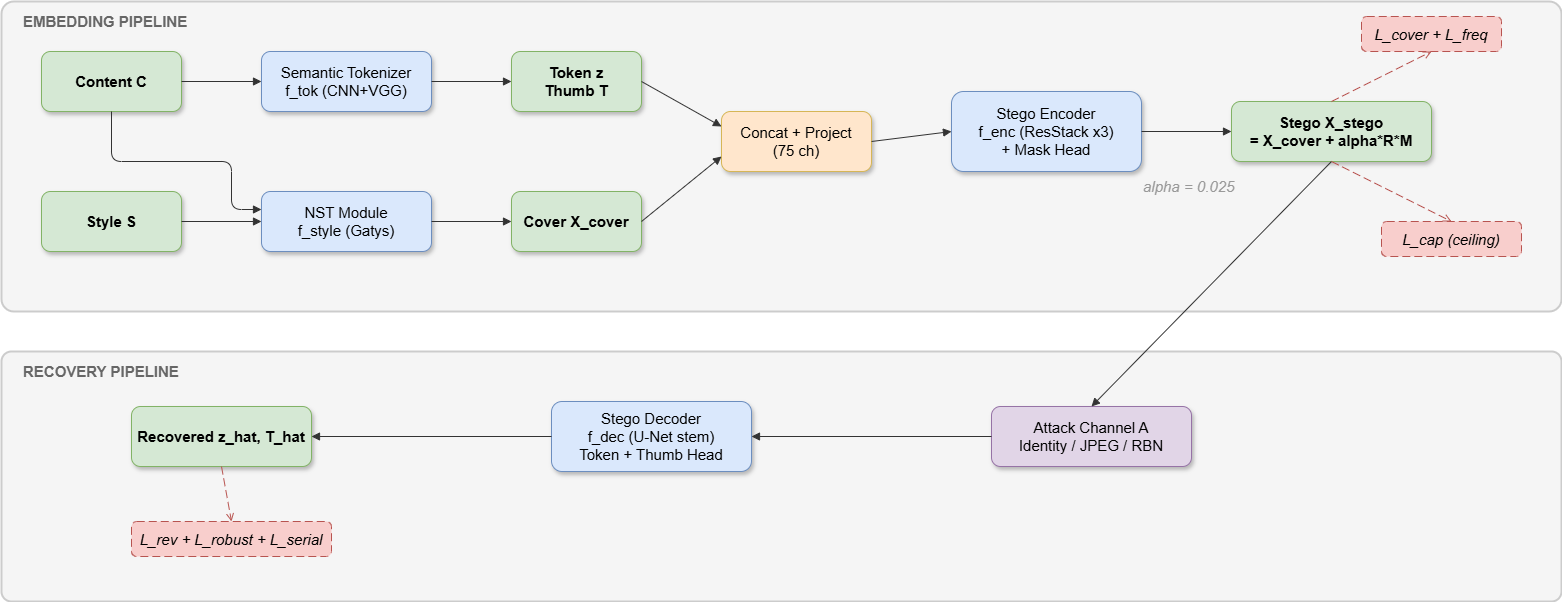
\includegraphics[width=\textwidth]{paper_assets/figure1_architecture.png}
    \caption{Frequency-guided semantic steganography network. Green nodes are tensors, blue nodes are learnable modules, orange nodes are differentiable operations, and purple nodes are stochastic but non-learnable. The dashed red boxes mark the three loss families that regulate the joint optimisation: a capacity-ceiling and prior block on the embedding side, a frequency / embedding-allocation block on the cover residual, and a reverse-extraction block, augmented by oracle distillation and a serial-source consistency term, on the recovery side.}
    \label{fig:architecture}
\end{figure*}

\section{Proposed Method}
\label{sec:method}

\subsection{Notation}
Scalars are written in plain math italic, vectors in bold lower case, and tensors in bold upper case. The cover image is $\mathbf{X}_{\text{cover}}\!\in\!\mathbb{R}^{3\times H\times W}$, the secret content is $\mathbf{C}\!\in\!\mathbb{R}^{3\times H\times W}$, and the painting reference is $\mathbf{S}$. The cover is obtained by an optimisation-based stylisation operator $f_{\text{style}}(\mathbf{C},\mathbf{S})$ that is held fixed during stego training. We denote by $\mathbf{z}\!\in\!\mathbb{R}^{d_{\text{tok}}\times g_{\text{tok}}\times g_{\text{tok}}}$ the semantic token used as payload, and by $\mathbf{T}\!\in\!\mathbb{R}^{3\times g_{\text{tok}}\times g_{\text{tok}}}$ the auxiliary thumbnail. In our default configuration we use $g_{\text{tok}}=32$ and $d_{\text{tok}}=64$ on $H\!=\!W\!=\!256$, and a smaller $g_{\text{tok}}=24,d_{\text{tok}}=24$ on $H\!=\!W\!=\!192$ for the lightweight ablation configuration.

\subsection{System Overview}
Our system consists of four modules: a semantic tokenizer $f_{\text{tok}}$, a stego encoder $f_{\text{enc}}$, a stego decoder $f_{\text{dec}}$, and a non-learnable attack channel $\mathcal{A}$. The first three are trained jointly. The attack channel enumerates three modes during training and is sampled stochastically at test time. Figure~\ref{fig:architecture} summarises the data flow. Both training and inference share the same flow, the only difference being that $\mathcal{A}$ samples from a single stochastic mode at test time but is enumerated at training time so that the decoder sees clean and degraded inputs in a balanced fashion.


\subsection{Cover Generation}
\label{sec:cover}
The cover is computed deterministically from $(\mathbf{C},\mathbf{S})$ by an optimisation-based stylisation operator $f_{\text{style}}$ in the spirit of Gatys~\cite{gatys}. Concretely, $f_{\text{style}}$ optimises a target image initialised at $\mathbf{C}$ for $T_{\text{nst}}$ steps with Adam~\cite{adam}, learning rate $\eta_{\text{nst}}\!=\!0.03$, content weight $1.0$ on the \texttt{conv\_3} feature map of an ImageNet-pretrained VGG-19~\cite{vgg}, and a style weight of $6\!\times\!10^{5}$ on the Gram matrices of \texttt{conv\_1}--\texttt{conv\_5}. We use $T_{\text{nst}}\!=\!45$ for the $256\!\times\!256$ benchmark protocol and $T_{\text{nst}}\!=\!120$ for the $192\!\times\!192$ CPU smoke run; $f_{\text{style}}$ is held frozen during the entire stego training, and the resulting covers are cached to disk per $(\mathbf{C},\mathbf{S})$ pair to keep the inner training loop deterministic.

\subsection{Semantic Tokenisation of the Secret}
\label{sec:tok}
A common pitfall of dense steganography is that the payload is itself spatial, so the encoder has to disturb a roughly equal number of pixels. We instead distil the secret into a compact representation. The tokenizer $f_{\text{tok}}$ comprises two parallel branches that are fused into a single token. The \emph{CNN branch} is a four-stage strided convolutional network: three $\text{Conv}_{3{\times}3}{+}\text{GroupNorm}{+}\text{GELU}$~\cite{gelu} blocks with stride two (channel widths $h/2 \!\to\! h \!\to\! h$, where $h\!=\!128$ in the GPU benchmark), followed by two residual blocks and a $1\!\times\!1$ projection to $d_{\text{tok}}$ channels, then adaptively pooled to $g_{\text{tok}}\!\times\!g_{\text{tok}}$. The \emph{VGG branch} extracts the \texttt{conv\_3} feature map from the frozen VGG-19 backbone~\cite{vgg} and projects it through two $1\!\times\!1$ convolutions ($256 \!\to\! h \!\to\! d_{\text{tok}}$), also adaptively pooled to $g_{\text{tok}}\!\times\!g_{\text{tok}}$. The two branch outputs are summed and activated with $\tanh$:
\begin{equation}
    \mathbf{z} = \tanh\!\left(\mathbf{z}_{\text{cnn}} + \mathbf{z}_{\text{vgg}}\right).
    \label{eq:tok}
\end{equation}
In parallel, a bilinearly resized RGB thumbnail $\mathbf{T}$ of the same spatial size is refined through a lightweight ConvBlock$+$ResBlock$+1\!\times\!1$ head with sigmoid activation, serving both as a soft anchor for the reverse decoder and as a regulariser that discourages pathological tokenisations. The semantic payload is therefore the pair $(\mathbf{z},\mathbf{T})$, with $\mathbf{z}\!\in\!\mathbb{R}^{64\times32\times32}$ in the GPU benchmark configuration; this corresponds to roughly $69$\,k floating-point values ($64\!\times\!32^{2}+3\!\times\!32^{2}$), approximately three times smaller than a $3\!\times\!256\!\times\!256$ secret image ($197$\,k values).

\subsection{Stego Encoder}
\label{sec:enc}
The encoder fuses the cover with five auxiliary feature maps to produce a texture-aware residual. The input tensor concatenates (i) the cover $\mathbf{X}_{\text{cover}}$ ($3$ ch.), (ii) the up-sampled token $\mathrm{up}(\mathbf{z})$ ($d_{\text{tok}}$ ch.), (iii) the up-sampled thumbnail $\mathrm{up}(\mathbf{T})$ ($3$ ch.), (iv) a two-channel Sobel edge map $\mathbf{E}=\mathrm{sobel}(\mathbf{X}_{\text{cover}})$, and (v) the cover--thumbnail difference $\mathbf{D}=\mathbf{X}_{\text{cover}}-\mathrm{up}(\mathbf{T})$ ($3$ ch.), yielding $3{+}d_{\text{tok}}{+}3{+}2{+}3=75$ input channels in the GPU configuration. The body is a ConvBlock$(75\!\to\!h)$ stem followed by three ResidualBlocks$(h)$, producing two parallel heads: a \emph{residual head} $\mathbf{R}=\tanh(\text{Conv}_{3\times3}(\cdot))$ and a \emph{mask head} $\mathbf{M}_{\text{learned}}=\sigma(\text{Conv}_{3\times3}(\cdot))$. The learned mask is modulated by a detached texture gate $\mathbf{G}$, computed from the normalised Sobel+DWT local-variance map of the cover (with a floor of $0.6$):
\begin{align}
    \mathbf{M} &= \mathbf{M}_{\text{learned}} \odot \left[\tau_{\text{floor}} + (1-\tau_{\text{floor}})\,\mathbf{G}\right], \label{eq:mask}\\
    \mathbf{X}_{\text{stego}} &= \mathrm{clip}_{[0,1]}\!\left(\mathbf{X}_{\text{cover}}+\alpha\,\sigma\,\mathbf{M}\odot\mathbf{R}\right),
    \label{eq:stego}
\end{align}
where $\alpha\!=\!0.025$ is a fixed residual scale, $\tau_{\text{floor}}\!=\!0.6$, and $\sigma\!\in\![1.02,1.30]$ at training ($\sigma_{\text{eval}}\!=\!1.36$). The masking mechanism steers perturbation energy towards textured regions and away from flat, perceptually salient areas. This mechanism directly complements the frequency loss. We use $h\!=\!128$ in the GPU configuration and $h\!=\!48$ in the CPU smoke configuration.

\subsection{Stego Decoder}
\label{sec:dec}
The decoder $f_{\text{dec}}$ is the dual of the tokenizer-plus-encoder. It consumes a $3\!\times\!H\!\times\!W$ stego image, applies three strided ConvBlocks, one ResStack, an adaptive pool to $g_{\text{tok}}\!\times\!g_{\text{tok}}$, and a $1\!\times\!1$ projection that produces $\hat{\mathbf{z}}$. A second $1\!\times\!1$ head additionally produces a sigmoidal thumbnail $\hat{\mathbf{T}}$ that we use as a reconstruction anchor. We use a single decoder rather than one decoder per attack mode, both for simplicity and to encourage representation transfer across distortion types.

\subsection{Attack Channel and Strength Curriculum}
\label{sec:attack}
The decoder is supervised under three modes of an attack channel $\mathcal{A}$:
\begin{align*}
    \mathcal{A}_{\text{id}}(\mathbf{X}) &= \mathbf{X}, \\
    \mathcal{A}_{\text{jpeg}}(\mathbf{X}) &= q\mathbf{X}+(1-q)\,\mathrm{AvgPool}_{3,1}(\mathbf{X}),\quad q=0.65, \\
    \mathcal{A}_{\text{rbn}}(\mathbf{X}) &= \mathrm{clip}_{[0,1]}(\mathbf{X}+\sigma_{n}\boldsymbol{\xi}),\quad \boldsymbol{\xi}\!\sim\!\mathcal{N}(0,I), \sigma_{n}=0.02.
\end{align*}
The JPEG-style proxy mimics the low-pass tendency of moderately compressed JPEGs without breaking gradient flow. The Gaussian mode adds zero-mean Gaussian noise. The strength scalar $\sigma_{\text{train}}$ is sampled per minibatch from $[1.02,1.30]$ to expose the decoder to a range of embedding magnitudes; at test time we always evaluate with $\sigma_{\text{eval}}=1.36$.

\subsection{Frequency-Guided Embedding}
\label{sec:freq}
A naive cover supervisor here would minimise the squared difference $\|\mathbf{X}_{\text{stego}}-\mathbf{X}_{\text{cover}}\|_2^2$. This penalises all spatial frequencies equally and, in practice, drains capacity from precisely the high-frequency bands where embedding is least visible. We therefore decompose the residual:
\begin{align}
    \boldsymbol{\Delta} &= \mathbf{X}_{\text{stego}}-\mathbf{X}_{\text{cover}}, \\
    \boldsymbol{\Delta}_{\text{LL}} &= \mathcal{U}\!\left(\mathcal{P}_{2,2}(\boldsymbol{\Delta})\right), \quad
    \boldsymbol{\Delta}_{\text{HH}} = \boldsymbol{\Delta}-\boldsymbol{\Delta}_{\text{LL}},
\end{align}
where $\mathcal{P}_{2,2}$ is a $2\!\times\!2$ average-pooling operator with stride two and $\mathcal{U}$ is a bilinear up-sampler back to the original resolution. The pair $(\mathcal{P}_{2,2},\mathcal{U})$ acts as a differentiable, parameter-free proxy for the $LL$ band of a one-level discrete wavelet transform with the Haar filter bank, and is markedly cheaper than a full DWT on every step. The frequency loss is then
\begin{equation}
    \mathcal{L}_{\text{freq}} = \mathbb{E}\!\left[\boldsymbol{\Delta}_{\text{LL}}^{\,2}\right] - \lambda_{\text{HH}}\,\mathbb{E}\!\left[\boldsymbol{\Delta}_{\text{HH}}^{\,2}\right],
    \label{eq:freq}
\end{equation}
with $\lambda_{\text{HH}}\!=\!0.1$. The first term penalises perturbations in the low-frequency band that carries colour and structure; the second is a small \emph{negative} term that explicitly rewards the model for placing energy in the high-frequency band, where the human visual system is least sensitive. We multiply $\mathcal{L}_{\text{freq}}$ by $\lambda_{\text{dwt}}\!=\!0.2$ in the joint objective.

In addition to $\mathcal{L}_{\text{freq}}$, we further supervise three coarse band-statistics of the residual against a smooth target shape derived from a texture mask $\mathbf{M}$ (the mask is computed as a normalised local-variance map of $\mathbf{X}_{\text{cover}}$ with floor $0.6$):
\begin{align}
    \mathcal{L}_{\text{embed}} = & \,\lambda_{\text{em-l}}\!\left\|\mathrm{LP}(\boldsymbol{\Delta})\right\|_1
    + \lambda_{\text{em-t}}\!\left\|(1-\mathbf{M})\odot\boldsymbol{\Delta}\right\|_1 \nonumber\\
    & + \lambda_{\text{em-h}}\!\left\|\boldsymbol{\Delta}-\mathrm{LP}(\boldsymbol{\Delta})\right\|_1,
    \label{eq:embed}
\end{align}
with $(\lambda_{\text{em-l}},\lambda_{\text{em-t}},\lambda_{\text{em-h}})=(0.5,0.3,0.12)$ and $\mathrm{LP}=\mathcal{U}\circ\mathcal{P}_{2,2}$. The first term suppresses low-frequency leakage; the second penalises perturbation outside textured regions; the third lightly regulates the high-frequency band so that it does not become arbitrarily noisy.

\subsection{Capacity-Ceiling Penalty}
\label{sec:ceil}
The capacity ceiling is the second key ingredient. A target cover PSNR $\tau_{\text{psnr}}$ corresponds to an MSE threshold $\epsilon = 10^{-\tau_{\text{psnr}}/10}$; for $\tau_{\text{psnr}}\!\approx\!39$\,dB we obtain $\epsilon\!\approx\!1.2\!\times\!10^{-4}$. We define
\begin{equation}
    \mathcal{L}_{\text{cap}} = \lambda_{\text{cov}}\,\mathbb{E}[\boldsymbol{\Delta}^2] + \lambda_{\text{ceil}} \left(\frac{\max\!\left(0,\mathbb{E}[\boldsymbol{\Delta}^2]-\epsilon\right)}{\epsilon}\right)^{\!2},
    \label{eq:cap}
\end{equation}
with $\lambda_{\text{cov}}\!=\!25$ and $\lambda_{\text{ceil}}\!=\!30$. The first term is a standard quadratic prior. The second is a one-sided, dimensionless quadratic explosion that activates only when the cover MSE exceeds $\epsilon$. Because the over-shoot is normalised by $\epsilon$ before being squared, the penalty grows extremely fast as soon as the encoder approaches the boundary. From a Lagrangian standpoint $\mathcal{L}_{\text{cap}}$ behaves like a soft barrier function, and the choice of $\epsilon$ becomes a direct control knob on the empirical cover PSNR; we verify this in Section~\ref{sec:ablation}. Figure~\ref{fig:ceiling} plots $\mathcal{L}_{\text{cap}}$ as a function of the cover MSE for the parameters used in this work, and illustrates the barrier shape directly: the loss is negligible below $\epsilon$ and increases sharply beyond it. To prevent the residual from degenerating to zero, we additionally regularise with a quadratic prior $\mathcal{L}_{\text{prior}}=\|\mathbf{R}\|_2^2$ (weight $\lambda_{\text{prior}}\!=\!4.5$) and a style-cover term $\mathcal{L}_{\text{style-cov}}$ (weight $\lambda_{\text{sc}}\!=\!0.06$) that asks $\mathbf{X}_{\text{stego}}$ to retain the Gram statistics of $\mathbf{X}_{\text{cover}}$.

\begin{figure}[t]
\centering
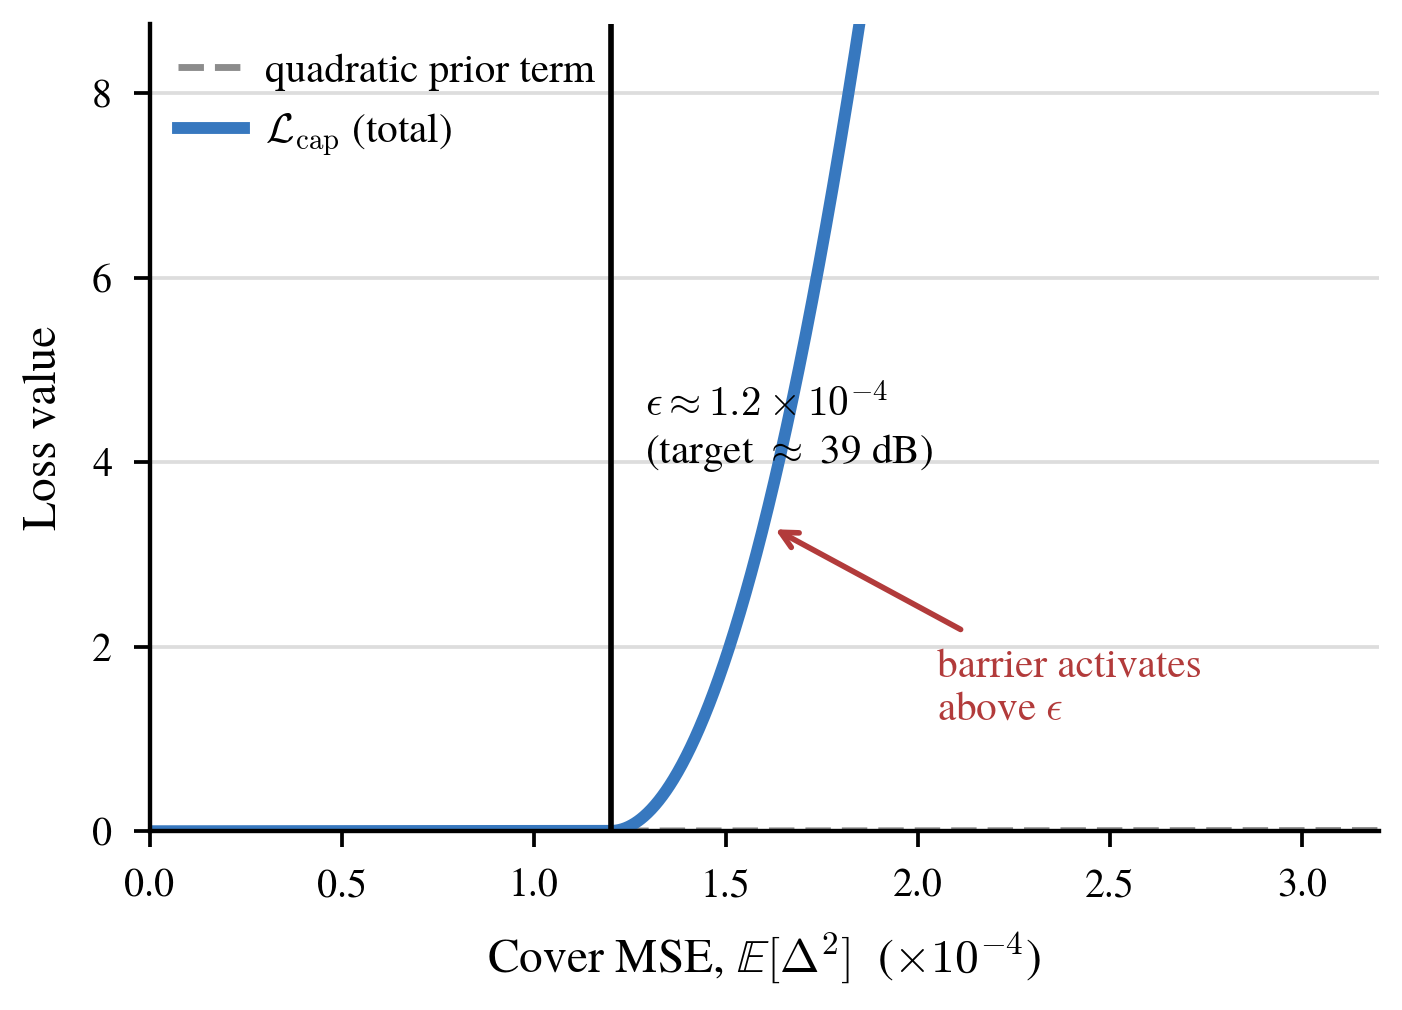
\includegraphics[width=0.70\textwidth]{paper_assets/ceiling_penalty.png}
\caption{The capacity-ceiling penalty $\mathcal{L}_{\text{cap}}$ (Eq.~\ref{eq:cap}) plotted against the cover MSE, using the parameters $\lambda_{\text{cov}}\!=\!25$, $\lambda_{\text{ceil}}\!=\!30$, $\epsilon\!\approx\!1.2\!\times\!10^{-4}$. The penalty is dominated by the quadratic prior below $\epsilon$ and by the barrier term above it, producing the soft-barrier shape referenced throughout Section~\ref{sec:exp}.}
\label{fig:ceiling}
\end{figure}

\subsection{Reverse Decoder Architecture}
\label{sec:revdec}
The reverse decoder $f_{\text{rev}}$ reconstructs the original content image $\mathbf{C}$ from the decoded token $\hat{\mathbf{z}}$ and thumbnail $\hat{\mathbf{T}}$. It consists of two cascaded sub-networks. The first, a \emph{Token Prior Decoder}, progressively up-samples the concatenation of $(\hat{\mathbf{z}},\hat{\mathbf{T}})$ ($d_{\text{tok}}{+}3$ channels at $g_{\text{tok}}\!\times\!g_{\text{tok}}$) through three stages ($32\!\to\!64\!\to\!128\!\to\!256$), each consisting of a ConvBlock and a ResidualBlock, producing a coarse prior $\mathbf{P}\!\in\!\mathbb{R}^{3\times H\times W}$ along with intermediate feature maps $\{\mathbf{f}_{128},\mathbf{f}_{256}\}$.

The second sub-network is a \emph{U-Net refinement decoder} that fuses the stego image with the prior. Its input concatenates seven feature groups: the stego image ($3$ ch.), the prior $\mathbf{P}$ ($3$ ch.), up-sampled thumbnail ($3$ ch.), up-sampled token ($d_{\text{tok}}$ ch.), Sobel edges of both the stego and the prior ($2{+}2$ ch.), and their absolute difference ($3$ ch.), yielding $3{+}3{+}3{+}64{+}2{+}2{+}3=80$ input channels. The U-Net has two encoder stages (stride-2 ConvBlocks), a two-block bottleneck, and two decoder stages with skip connections that also incorporate the prior feature maps $\mathbf{f}_{128}$ and $\mathbf{f}_{256}$. Two output heads produce a blend map $\boldsymbol{\beta}=\sigma(\text{Conv}_{3\times3}(\cdot))$ and a delta $\boldsymbol{\delta}=\tanh(\text{Conv}_{3\times3}(\cdot))$:
\begin{equation}
    \hat{\mathbf{C}} = \mathrm{clip}_{[0,1]}\!\Big(\boldsymbol{\beta}\odot\mathbf{P} + (1{-}\boldsymbol{\beta})\odot\mathrm{up}(\hat{\mathbf{T}}) + \gamma\,\boldsymbol{\delta}\Big),
    \label{eq:revdec}
\end{equation}
where $\gamma\!=\!0.22$ (\texttt{reverse\_refine\_scale}). This design lets the network smoothly interpolate between the prior and the thumbnail while applying a learned residual correction.






\subsection{Reverse Loss and Oracle Distillation}
\label{sec:rev}
The reverse loss combines three attack-conditioned terms:
\begin{equation}
    \mathcal{L}_{\text{rev}} = \lambda_{\text{r}}\,\mathcal{L}_{\text{rev,id}} + \lambda_{\text{rR}}\,\mathcal{L}_{\text{rev,rbn}} + \lambda_{\text{rJ}}\,\mathcal{L}_{\text{rev,jpeg}},
    \label{eq:rev}
\end{equation}
where each $\mathcal{L}_{\text{rev},*}$ is a composite of Charbonnier, perceptual (VGG conv\_1--3), edge, low-frequency, FFT-magnitude and colour-mean losses between the reconstructed content and the original, augmented by a content--cover margin term that encourages the reconstruction to be closer to the content than to the cover in feature space. $(\lambda_{\text{r}},\lambda_{\text{rR}},\lambda_{\text{rJ}})=(25,12,12)$. We additionally maintain an \emph{oracle reverse} signal: the reverse decoder is also run with the \emph{ground-truth} token and thumbnail (detached) to produce a clean reference $\hat{\mathbf{C}}^{\star}$; matching the attack-conditioned reconstructions to $\hat{\mathbf{C}}^{\star}$ stabilises decoding:
\begin{equation}
    \mathcal{L}_{\text{oracle}} = \lambda_{\text{or}}\!\left\|\hat{\mathbf{C}}-\hat{\mathbf{C}}^{\star}\right\|_1
    + \lambda_{\text{od}}\!\left\|\hat{\mathbf{C}}_{\text{robust}}-\hat{\mathbf{C}}^{\star}\right\|_1, \label{eq:oracle}
\end{equation}
with $\lambda_{\text{or}}\!=\!2.6$ and $\lambda_{\text{od}}\!=\!1.4$. A token consistency term $\mathcal{L}_{\text{tok-c}}$ (weight $0.25$) and a thumbnail consistency term $\mathcal{L}_{\text{thumb}}$ (weight $3.0$) together with $\mathcal{L}_{\text{tok}}=\|\hat{\mathbf{z}}-\mathbf{z}\|_2^2$ (weight $3.0$) close out the reverse-side supervision.

\subsection{Serial-Source Consistency and Future-Pass Sampling}
\label{sec:serial}
A defining requirement of self-contained stylisation is that the stego image survives one or two further re-stylisations $\mathbf{X}_{k}\!=\!f_{\text{style}}(\mathbf{X}_{k-1},\mathbf{S}_{k})$. We supervise this by adding a \emph{serial-source} consistency loss
\begin{equation}
    \mathcal{L}_{\text{ser}} = \lambda_{\text{ser}}\!\left\|f_{\text{dec}}\!\left(\beta\mathbf{X}_{\text{stego}}+(1-\beta)\mathbf{X}_{2}\right)-\mathbf{z}\right\|_2^{2},
    \label{eq:ser}
\end{equation}
with $\lambda_{\text{ser}}\!=\!1.5$ and a blending coefficient $\beta\!=\!0.7$ (\texttt{serial\_prior\_blend}\,$=0.3$). Equation~(\ref{eq:ser}) is evaluated on a sample drawn from the precomputed cache of \emph{direct-2} re-stylisations. Because materialising additional NST passes is expensive, we further enable a stochastic \emph{future pass}: with probability $p_{\text{f}}\!=\!0.005$ each step performs an extra forward pass through one of the precomputed direct-2 / direct-3 covers, and adds the resulting reverse loss with weight $w_{\text{f}}\!=\!0.04$. The combination follows an empirical trade-off observed in our preliminary experiments: a too aggressive $p_{\text{f}}$ destabilises the cover, while a vanishing $p_{\text{f}}$ removes serial-step generalisation entirely.

\subsection{Joint Objective and Training Schedule}
\label{sec:total}
The full per-step objective gathers all losses introduced so far:
\begin{equation}
\begin{aligned}
\mathcal{L} =&\, \mathcal{L}_{\text{cap}} + \lambda_{\text{prior}}\mathcal{L}_{\text{prior}} + \lambda_{\text{sc}}\mathcal{L}_{\text{style-cov}} \\
& + \lambda_{\text{dwt}}\mathcal{L}_{\text{freq}} + \mathcal{L}_{\text{embed}} \\
& + \mathcal{L}_{\text{rev}} + \mathcal{L}_{\text{oracle}} + \mathcal{L}_{\text{ser}} \\
& + \lambda_{\text{tok}}\mathcal{L}_{\text{tok}} + \lambda_{\text{tc}}\mathcal{L}_{\text{tok-c}} + \lambda_{\text{th}}\mathcal{L}_{\text{thumb}} \\
& + \lambda_{\text{cs}}\mathcal{L}_{\text{cons}} + \lambda_{\text{q}}\mathcal{L}_{\text{quant}}.
\end{aligned}
\label{eq:total}
\end{equation}
Here $\mathcal{L}_{\text{cons}}$ enforces $f_{\text{dec}}\!\circ\!f_{\text{enc}}$ idempotency on the cover when no token is injected (weight $1.6$), and $\mathcal{L}_{\text{quant}}$ is a small entropy-coding regulariser on $\mathbf{z}$ (weight $0.12$) that we found to stabilise serial extraction.

By this point Eq.~(\ref{eq:total}) has accumulated thirteen terms across five subsections; Table~\ref{tab:losscheat} collects them in one place as a reference for the rest of the paper.

\begin{table}[t]
\centering
\caption{Reference summary of every term in the joint objective, Eq.~(\ref{eq:total}). Weights are the values used in the GPU benchmark configuration.}
\label{tab:losscheat}
\setlength{\tabcolsep}{6pt}
\small
\begin{tabular}{lcl}
\toprule
\textbf{Term} & \textbf{Weight} & \textbf{Role} \\
\midrule
$\mathcal{L}_{\text{cap}}$ & $\lambda_{\text{cov}}\!=\!25,\lambda_{\text{ceil}}\!=\!30$ & cover-MSE soft barrier (Sec.~\ref{sec:ceil}) \\
\rowcolor{rowshade}
$\mathcal{L}_{\text{prior}}$ & $4.5$ & keeps residual non-zero \\
$\mathcal{L}_{\text{style-cov}}$ & $0.06$ & retains cover's Gram statistics \\
\rowcolor{rowshade}
$\mathcal{L}_{\text{freq}}$ & $\lambda_{\text{dwt}}\!=\!0.2$ & pushes energy to high-freq band \\
$\mathcal{L}_{\text{embed}}$ & see Eq.~(\ref{eq:embed}) & band-localised allocation shape \\
\rowcolor{rowshade}
$\mathcal{L}_{\text{rev}}$ & $(25,12,12)$ & attack-conditioned reverse loss \\
$\mathcal{L}_{\text{oracle}}$ & $(2.6, 1.4)$ & distils clean-token reconstruction \\
\rowcolor{rowshade}
$\mathcal{L}_{\text{ser}}$ & $1.5$ & serial-source consistency \\
$\mathcal{L}_{\text{tok}}$ & $3.0$ & token regression, $\|\hat{\mathbf{z}}-\mathbf{z}\|_2^2$ \\
\rowcolor{rowshade}
$\mathcal{L}_{\text{tok-c}}$ & $0.25$ & token consistency \\
$\mathcal{L}_{\text{thumb}}$ & $3.0$ & thumbnail consistency \\
\rowcolor{rowshade}
$\mathcal{L}_{\text{cons}}$ & $1.6$ & $f_{\text{dec}}\!\circ\!f_{\text{enc}}$ idempotency \\
$\mathcal{L}_{\text{quant}}$ & $0.12$ & entropy-coding regulariser on $\mathbf{z}$ \\
\bottomrule
\end{tabular}
\end{table}

Training proceeds in three phases that share Eq.~(\ref{eq:total}) but rescale the reverse and serial-source weights through a phase mask $\boldsymbol{\phi}_{e}$:
\begin{itemize}
    \item \textbf{Fidelity-lock} (epochs $1$--$15$): $\boldsymbol{\phi}$ emphasises $\mathcal{L}_{\text{cap}}$, $\mathcal{L}_{\text{prior}}$, $\mathcal{L}_{\text{freq}}$ and $\mathcal{L}_{\text{embed}}$ at full weight; reverse and serial weights are damped by a factor of $0.6$. The phase resets the cover model around the target PSNR before any reverse pressure is applied.
    \item \textbf{Robust-push} (epochs $16$--$28$): reverse, oracle and consistency losses are restored to full weight; serial-source is still attenuated.
    \item \textbf{SOTA-refine} (epochs $29$--$E$): all weights are at $1\!\times\!\boldsymbol{\phi}$, and the future-pass sampler is enabled. A baseline guard activates from epoch $35$: if the validation score $V$ has not improved by more than $0.02$ within $8$ epochs, the optimiser falls back to the best checkpoint.
\end{itemize}
Figure~\ref{fig:phasetimeline} summarises this schedule graphically, indicating which loss terms are emphasised or damped in each phase and marking the epochs at which the baseline guard activates and the reported checkpoint is selected.

\begin{figure}[t]
\centering
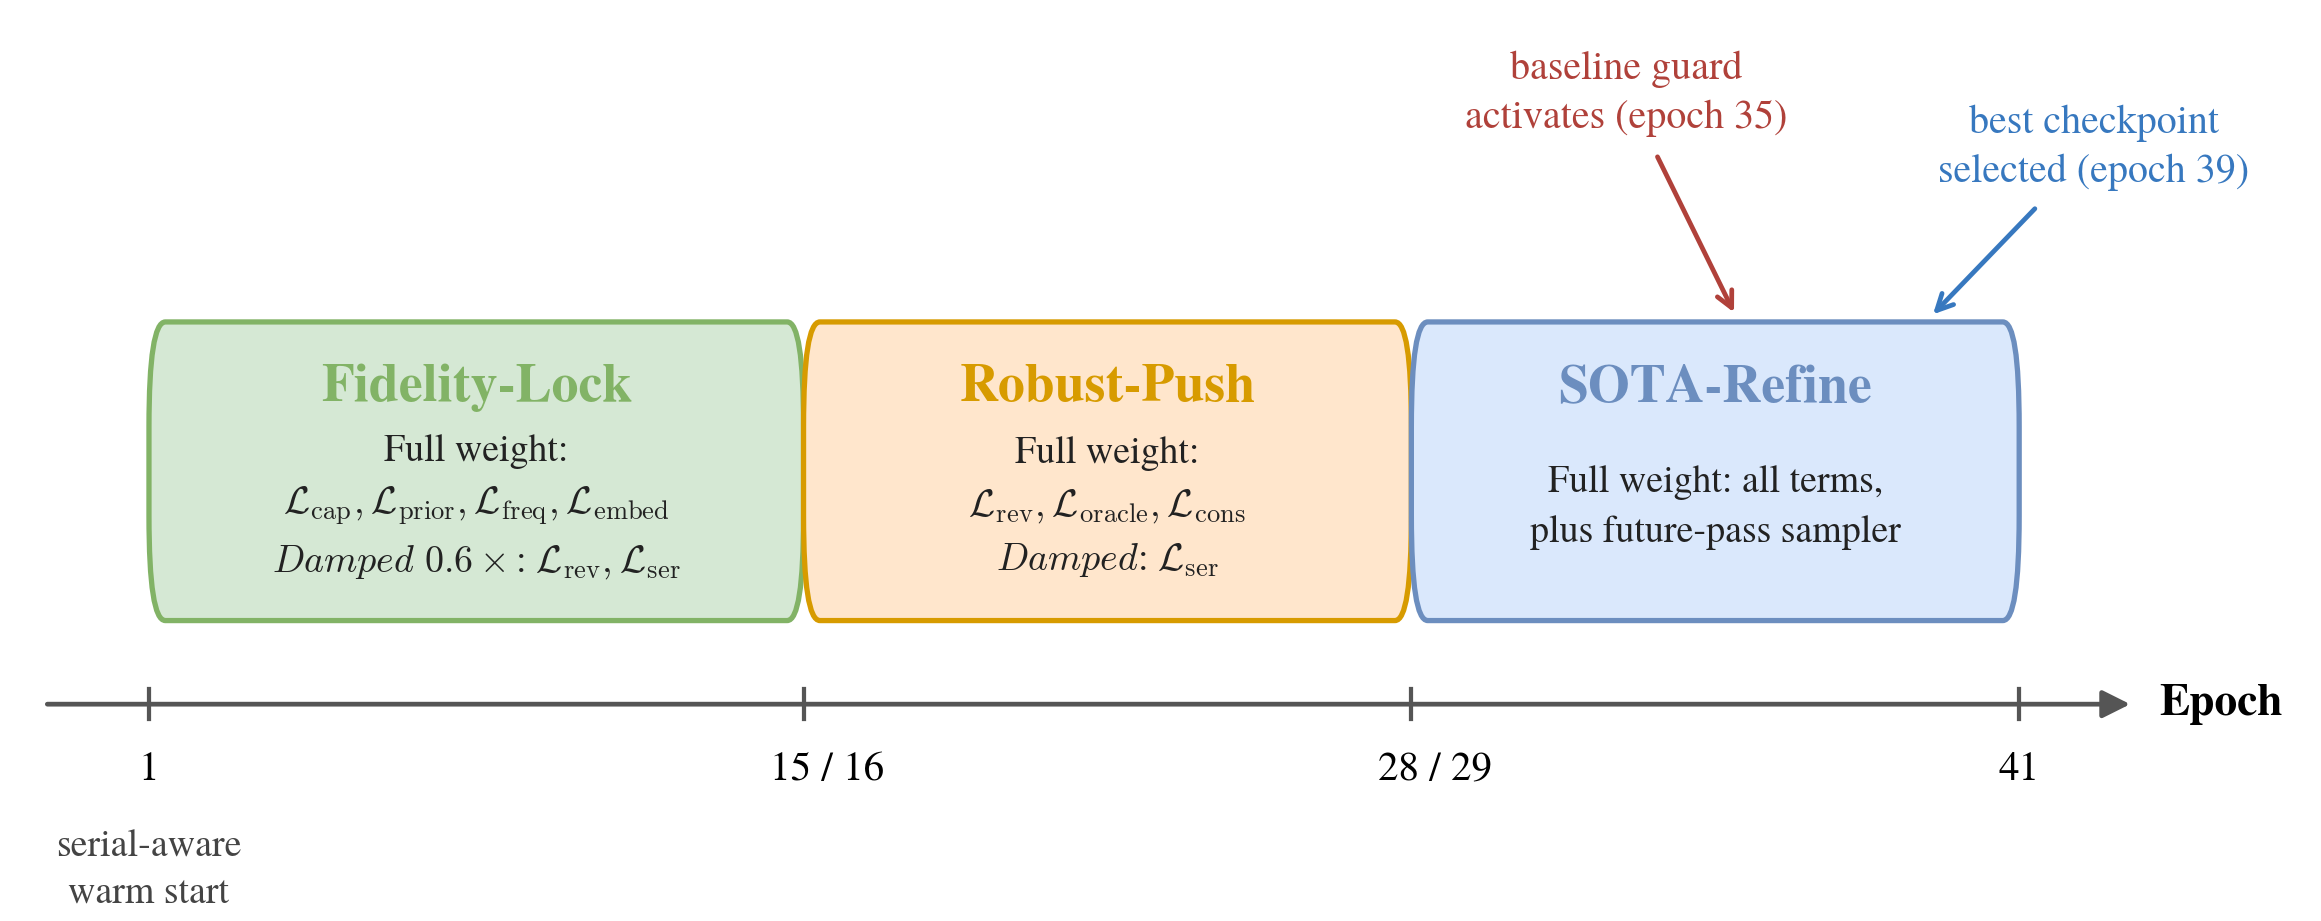
\includegraphics[width=0.92\textwidth]{paper_assets/phase_timeline.png}
\caption{The three-phase training schedule used throughout this work. Each phase rescales a subset of the loss terms in Eq.~(\ref{eq:total}) via the phase mask $\boldsymbol{\phi}_e$; the reported checkpoint (epoch $39$) falls within the \emph{sota-refine} phase, after the baseline guard has activated.}
\label{fig:phasetimeline}
\end{figure}

We monitor the composite validation score $V = 0.45\,V_{\text{rev,clean}} + 0.20\,V_{\text{rev,rbn}} + 0.20\,V_{\text{rev,jpeg}} + 0.075\,V_{\text{ser2}} + 0.075\,V_{\text{ser3}} + 1.0$ and select the checkpoint with the lowest $V$. The schedule is also summarised in Algorithm~\ref{alg:train}.

\begin{algorithm}[t]
\caption{Frequency-guided semantic steganography training.}
\label{alg:train}
\begin{algorithmic}[1]
\Require Cover generator $f_{\text{style}}$, modules $f_{\text{tok}}, f_{\text{enc}}, f_{\text{dec}}$.
\Require Hyper-parameters $(\epsilon, \lambda_{\text{cov}}, \lambda_{\text{ceil}}, \lambda_{\text{rev}}, \lambda_{\text{dwt}}, \alpha,\sigma)$ and warm-start $\theta_{0}$.
\State Initialise $(f_{\text{tok}}, f_{\text{enc}}, f_{\text{dec}})\leftarrow\theta_{0}$ from a serial-aware warm-start checkpoint.
\For{epoch $e=1,\dots,E$}
    \State $\boldsymbol{\phi}_{e}\gets$ phase weights for epoch $e$ (see Sec.~\ref{sec:total})
    \For{mini-batch $(\mathbf{C},\mathbf{S},\mathbf{X}_{2},\mathbf{X}_{3})$}
        \State $\mathbf{X}_{\text{cover}}\gets f_{\text{style}}(\mathbf{C},\mathbf{S})$ (cached)
        \State $(\mathbf{z},\mathbf{T})\gets f_{\text{tok}}(\mathbf{C})$
        \State Sample $\sigma_{\text{train}}\!\in\![1.02,1.30]$
        \State $\mathbf{X}_{\text{stego}}\gets$ Eq.~(\ref{eq:stego})
        \State Compute $\mathcal{L}_{\text{cap}}, \mathcal{L}_{\text{freq}}, \mathcal{L}_{\text{embed}}$ via Eqs.~(\ref{eq:cap})--(\ref{eq:embed}).
        \State Compute $\mathcal{L}_{\text{rev}}$ over $\{\mathcal{A}_{\text{id}},\mathcal{A}_{\text{rbn}},\mathcal{A}_{\text{jpeg}}\}$.
        \State Compute $\mathcal{L}_{\text{oracle}}$ from a detached re-tokenisation of $\mathbf{X}_{\text{stego}}$.
        \State Compute $\mathcal{L}_{\text{ser}}$ on a blended cover with $\mathbf{X}_{2}$.
        \If{$U(0,1) < p_{\text{f}}$ and phase = sota-refine}
            \State Add a future-pass term on a random sample from $\{\mathbf{X}_{2},\mathbf{X}_{3}\}$ with weight $w_{\text{f}}$.
        \EndIf
        \State $\mathcal{L}\gets$ Eq.~(\ref{eq:total}), reweighted by $\boldsymbol{\phi}_{e}$.
        \State Update $\theta$ by Adam (lr $6.5\!\times\!10^{-5}$, wd $10^{-5}$).
    \EndFor
    \State Evaluate $V$ on the held-out partition; update best checkpoint; trigger baseline guard if needed.
\EndFor
\end{algorithmic}
\end{algorithm}

\section{Experimental Results}
\label{sec:exp}

\subsection{Datasets and Protocol}
\label{sec:proto}
% SOURCE: run_summary.json (protocol), manifest_splits.csv
We build the protocol around the official COCO~val2017~\cite{coco} split paired with the five exemplar paintings shipped with the AdaIN~\cite{adain} repository (\textit{antimonocromatismo}, \textit{impronte\_d\_artista}, \textit{picasso\_self\_portrait}, \textit{trial}, \textit{woman\_with\_hat\_matisse}). The full COCO~val2017 set is downloaded and deterministically split with \texttt{SEED=42}: the training partition uses $300$ COCO contents $\times$ $5$ styles $= 1\,500$ pairs, and the held-out evaluation partition uses $120$ unseen COCO contents $\times$ $5$ styles $= 600$ pairs. At evaluation time, the trained encoder/decoder pair is run in pure inference mode on each of these $600$ unseen content--style pairs: a fresh cover is rendered by $f_{\text{style}}(\mathbf{C},\mathbf{S})$ for each unseen COCO content $\mathbf{C}$ paired with each of the five painting references $\mathbf{S}$, the encoder embeds the semantic token, and the decoder is queried under the three attack modes of $\mathcal{A}$ (Section~\ref{sec:attack}); none of these content--style pairs is seen during training. The protocol is content-agnostic in the sense that any additional COCO image can be substituted for inference without retraining. Each pair is further augmented with two precomputed serial covers (\textit{direct-2}, \textit{direct-3}) drawn from a deterministic rotation over the style list, so that the serial-source loss can be evaluated without invoking $f_{\text{style}}$ during training. All images are resized to $256\!\times\!256$ for the GPU benchmark protocol and to $192\!\times\!192$ for the CPU smoke run. The cover generator is held fixed at training time and applied as in Section~\ref{sec:cover}, with its outputs cached per pair.

\subsection{Implementation Details}
\label{sec:impl}
% SOURCE: run_summary.json (protocol, history, best_epoch)
The tokenizer, encoder and decoder are trained jointly with Adam~\cite{adam}, learning rate $6.5\!\times\!10^{-5}$, weight decay $10^{-5}$ and a cosine schedule. The benchmark protocol was trained end-to-end on a single \emph{NVIDIA A100} GPU rented through Google~Colab; mixed-precision execution is disabled, so the recorded numbers correspond to FP32 training. Training runs for $41$ epochs starting from a serial-aware warm-start checkpoint. On the A100, one full epoch over the $1\,500$ training pairs takes approximately $870$\,s, so a complete training schedule requires approximately $9.9$ hours of wall-clock time. The evaluation strength is $\sigma_{\text{eval}}=1.36$. The hyper-parameters of the loss are set to $\epsilon\!=\!1.2\!\times\!10^{-4}$, $\lambda_{\text{cov}}\!=\!25$, $\lambda_{\text{ceil}}\!=\!30$, $\lambda_{\text{prior}}\!=\!4.5$, $\lambda_{\text{sc}}\!=\!0.06$, $\lambda_{\text{dwt}}\!=\!0.2$, $\lambda_{\text{HH}}\!=\!0.1$, $(\lambda_{\text{em-l}},\lambda_{\text{em-t}},\lambda_{\text{em-h}})\!=\!(0.5,0.3,0.12)$, $(\lambda_{\text{r}},\lambda_{\text{rR}},\lambda_{\text{rJ}})\!=\!(25,12,12)$, $(\lambda_{\text{or}},\lambda_{\text{od}})\!=\!(2.6,1.4)$, $\lambda_{\text{ser}}\!=\!1.5$, $\beta\!=\!0.7$, $(\lambda_{\text{tok}},\lambda_{\text{tc}},\lambda_{\text{th}},\lambda_{\text{cs}},\lambda_{\text{q}})\!=\!(3.0,0.25,3.0,1.6,0.12)$, $\alpha\!=\!0.025$, $p_{\text{f}}\!=\!0.005$, $w_{\text{f}}\!=\!0.04$. Training proceeds in three phases: \emph{fidelity-lock} (epochs $1$--$15$), \emph{robust-push} (epochs $16$--$28$), and \emph{sota-refine} (epochs $29$--$41$). The best checkpoint reported throughout this section was selected at epoch~$39$ with validation score $V^{\star}\!=\!3.549$. The CPU smoke run shares all of the loss formulation but uses smaller capacity ($h\!=\!48,d_{\text{tok}}\!=\!24,g_{\text{tok}}\!=\!24$) and a fixed scalar batch ($60$ epochs, single content/style pair) on a single CPU thread of an ordinary desktop machine, and is the sole source of the inference timings reported in Section~\ref{sec:inference}.

\subsection{Cover-Side Fidelity and Token Robustness}
\label{sec:exp_coco}
% SOURCE: run_summary.json (cover_metrics_mean), token_summary.csv, paper_numbers_overview.json
Table~\ref{tab:cover} reports cover-side fidelity and token-side robustness on the held-out evaluation partition, expressed as mean$\pm$std over the $600$ evaluation pairs at evaluation strength $\sigma_{\text{eval}}\!=\!1.36$. The model attains $39.61$\,dB cover PSNR, $0.9914$ SSIM, and $0.0195$ LPIPS, exceeding the $33$--$36$\,dB typically reported by style-transfer steganography approaches~\cite{stylestegan2023,sst2024,stisgan2026}. The standard deviation of the cover PSNR remains below $0.35$\,dB, indicating that the capacity ceiling produces a stable empirical bound rather than a high-variance optimum. Robustness follows a similar pattern: the token MSE varies by less than $1\!\times\!10^{-4}$ across the three attack modes, which translates into reverse SSIM under attack that is virtually indistinguishable from clean-channel decoding (Table~\ref{tab:reverse}).

\begin{table}[t]
\centering
% SOURCE: run_summary.json (cover_metrics_mean), token_summary.csv
\caption{Cover-side fidelity and token-side robustness on the COCO~val2017 evaluation split ($600$ content--style pairs, $\sigma_{\text{eval}}=1.36$, best epoch~$39$).}
\label{tab:cover}
\setlength{\tabcolsep}{8pt}
\begin{tabular}{l c}
\toprule
\textbf{Quantity} & \textbf{mean $\pm$ std} \\
\midrule
Cover L2          & $1.10\!\times\!10^{-4} \pm 0.00\!\times\!10^{-4}$ \\
\rowcolor{rowshade}
Cover SSIM        & $0.9914 \pm 0.0030$ \\
Cover LPIPS       & $0.0195 \pm 0.0081$ \\
\rowcolor{rowshade}
Cover PSNR (dB)   & $\mathbf{39.6074 \pm 0.3532}$ \\
\midrule
Token MSE (clean) & $0.0133 \pm 0.0043$ \\
\rowcolor{rowshade}
Token MSE (RBN)   & $0.0133 \pm 0.0045$ \\
Token MSE (JPEG)  & $0.0132 \pm 0.0044$ \\
\bottomrule
\end{tabular}
\end{table}

\subsection{Reverse Style Transfer}
\label{sec:exp_reverse}
% SOURCE: paper_table_main.csv (rows 2-6)
This experiment isolates the contribution of the semantic token to reverse recovery. Table~\ref{tab:reverse} compares a content-free \emph{naive reverse} baseline (which re-stylises the stego image back through $f_{\text{style}}$ without access to any embedded payload) against four token-conditioned variants of our decoder. The token-conditioned variants yield a substantial improvement in reverse SSIM, from $0.5234$ to $0.8070$ on the clean channel, and to $0.8136$ when the \emph{oracle} variant is given the ground-truth token. PSNR improves correspondingly, from $22.25$\,dB to $27.46$\,dB, a gain of $5.21$\,dB attributable to the token alone. Notably, the token-conditioned decoder is largely insensitive to which attack it encounters at inference time: SSIM varies only from $0.8070$ (clean) to $0.7884$ (Gaussian) to $0.7898$ (JPEG), indicating that the reverse decoder generalises consistently across the three attack modes. LPIPS improves in the same direction, from $0.189$ (naive) to $0.122$ (clean), indicating that the improvement is perceptual as well as numerical.

\begin{table}[t]
\centering
% SOURCE: paper_table_main.csv (rows 2-6)
\caption{Reverse style transfer comparison ($600$ evaluation pairs, $\sigma_{\text{eval}}\!=\!1.36$). \textit{naive\_reverse} is a content-free re-stylisation baseline; \textit{token\_*} variants use our reverse decoder. \textit{oracle} reads the ground-truth token, the others operate on the decoded token after identity / RBN / JPEG distortion.}
\label{tab:reverse}
\setlength{\tabcolsep}{4pt}
\footnotesize
\begin{tabular}{lcccc}
\toprule
\textbf{Method} & \textbf{L2}\,$\downarrow$ & \textbf{SSIM}\,$\uparrow$ & \textbf{LPIPS}\,$\downarrow$ & \textbf{PSNR}\,$\uparrow$ \\
\midrule
naive\_reverse        & $0.0065\pm0.0029$ & $0.5234\pm0.0852$ & $0.1889\pm0.0905$ & $22.25\pm1.71$ \\
\rowcolor{rowshade}
token\_reverse\_clean & $0.0022\pm0.0015$ & $\mathbf{0.8070\pm0.0858}$ & $0.1216\pm0.0799$ & $\mathbf{27.46\pm2.68}$ \\
token\_reverse\_rbn   & $0.0027\pm0.0019$ & $0.7884\pm0.0931$ & $0.1514\pm0.0893$ & $26.54\pm2.75$ \\
\rowcolor{rowshade}
token\_reverse\_jpeg  & $0.0025\pm0.0018$ & $0.7898\pm0.0968$ & $0.1467\pm0.0909$ & $26.97\pm2.78$ \\
\textbf{token\_reverse\_oracle} & $0.0021\pm0.0015$ & $\mathbf{0.8136\pm0.0852}$ & $\mathbf{0.1135\pm0.0768}$ & $27.63\pm2.82$ \\
\bottomrule
\end{tabular}
\end{table}

\subsection{Serial Style Transfer (Direct-2 and Direct-3)}
\label{sec:exp_serial}
% SOURCE: paper_table_main.csv (rows 7-14)
Table~\ref{tab:serial2} and Table~\ref{tab:serial3} report recovery quality after one extra re-stylisation (\emph{serial-2}) and two extra re-stylisations (\emph{serial-3}), respectively, and two consistent patterns emerge. First, SSIM is the only metric for which the naive baseline slightly exceeds the proposed method ($0.4966$ vs.\ $0.4943$ at serial-2); however, this margin is small and is reversed on every other metric: L2 decreases from $0.0090$ to $0.0078$, LPIPS from $0.1945$ to $0.1577$, and PSNR increases from $20.64$ to $21.41$\,dB. Token-conditioned recovery therefore outperforms the naive baseline on three of four metrics at both serial steps. Second, the token-conditioned variants exhibit markedly greater \emph{stability}: their SSIM standard deviation is consistently lower than that of the naive baseline. This represents a favourable trade-off for a steganographic system, exchanging a marginal reduction in SSIM for substantially more predictable and perceptually consistent output.

\begin{table}[t]
\centering
% SOURCE: paper_table_main.csv (rows 7-14)
\caption{Two-step serial style transfer (\emph{serial-2}, $600$ pairs). ``blend'' rows use the proposed blended serial-source; ``render'' rows additionally re-render through $f_{\text{style}}$ at test time. All token/blend rows use our reverse decoder.}
\label{tab:serial2}
\setlength{\tabcolsep}{4pt}
\footnotesize
\begin{tabular}{lcccc}
\toprule
\textbf{Method} & \textbf{L2}\,$\downarrow$ & \textbf{SSIM}\,$\uparrow$ & \textbf{LPIPS}\,$\downarrow$ & \textbf{PSNR}\,$\uparrow$ \\
\midrule
naive                & $0.0090\pm0.0027$ & $0.4966\pm0.0936$ & $0.1945\pm0.0725$ & $20.64\pm1.26$ \\
\rowcolor{rowshade}
token\_clean          & $\mathbf{0.0078\pm0.0030}$ & $0.4943\pm0.0844$ & $\mathbf{0.1577\pm0.0585}$ & $\mathbf{21.41\pm1.65}$ \\
token\_jpeg           & $0.0081\pm0.0031$ & $0.4796\pm0.0831$ & $0.1662\pm0.0591$ & $21.23\pm1.69$ \\
\rowcolor{rowshade}
blend\_render\_clean  & $0.0083\pm0.0031$ & $0.4738\pm0.0827$ & $0.1836\pm0.0629$ & $21.10\pm1.63$ \\
blend\_clean          & $0.0081\pm0.0031$ & $0.4795\pm0.0834$ & $0.1715\pm0.0612$ & $21.20\pm1.64$ \\
\rowcolor{rowshade}
blend\_rbn            & $0.0087\pm0.0033$ & $0.4615\pm0.0816$ & $0.1815\pm0.0624$ & $20.89\pm1.64$ \\
blend\_jpeg           & $0.0085\pm0.0032$ & $0.4647\pm0.0824$ & $0.1802\pm0.0621$ & $21.02\pm1.67$ \\
\bottomrule
\end{tabular}
\end{table}

\begin{table}[t]
\centering
% SOURCE: paper_table_main.csv (rows 15-22)
\caption{Three-step serial style transfer (\emph{serial-3}, $600$ pairs). Same conventions as Table~\ref{tab:serial2}; compare row-by-row against it to see the extra degradation from the second re-stylisation pass.}
\label{tab:serial3}
\setlength{\tabcolsep}{4pt}
\footnotesize
\begin{tabular}{lcccc}
\toprule
\textbf{Method} & \textbf{L2}\,$\downarrow$ & \textbf{SSIM}\,$\uparrow$ & \textbf{LPIPS}\,$\downarrow$ & \textbf{PSNR}\,$\uparrow$ \\
\midrule
naive                & $0.0113\pm0.0033$ & $0.4548\pm0.0767$ & $0.2378\pm0.0684$ & $19.64\pm1.27$ \\
\rowcolor{rowshade}
token\_clean          & $\mathbf{0.0091\pm0.0035}$ & $0.4500\pm0.0881$ & $\mathbf{0.1885\pm0.0627}$ & $\mathbf{20.71\pm1.69}$ \\
token\_jpeg           & $0.0094\pm0.0036$ & $0.4376\pm0.0872$ & $0.1984\pm0.0635$ & $20.58\pm1.70$ \\
\rowcolor{rowshade}
blend\_render\_clean  & $0.0102\pm0.0038$ & $0.4192\pm0.0849$ & $0.2260\pm0.0666$ & $20.23\pm1.64$ \\
blend\_clean          & $0.0098\pm0.0037$ & $0.4278\pm0.0864$ & $0.2090\pm0.0654$ & $20.38\pm1.66$ \\
\rowcolor{rowshade}
blend\_rbn            & $0.0108\pm0.0040$ & $0.4046\pm0.0846$ & $0.2196\pm0.0657$ & $19.98\pm1.64$ \\
blend\_jpeg           & $0.0102\pm0.0038$ & $0.4155\pm0.0856$ & $0.2196\pm0.0658$ & $20.25\pm1.68$ \\
\bottomrule
\end{tabular}
\end{table}

\subsection{Ablation of the Loss Terms}
\label{sec:ablation}
To isolate the contribution of each design choice, we conducted a controlled ablation on a CPU smoke configuration, training the same scaffold for $50$ epochs on a single content/style pair under all four combinations of $(\text{ceiling on/off}, \text{frequency loss on/off})$ (Table~\ref{tab:ablation}). Three observations follow. First, removing the capacity ceiling from the joint objective reduces cover PSNR by $5.76$\,dB ($41.37\to35.61$); the network continues to encode the token successfully, but no longer guarantees a high-quality cover. Second, the frequency loss in isolation is essentially neutral with respect to cover PSNR: it does not bound the residual magnitude, only its spectral allocation, so the PSNR and MSE values are numerically identical to the baseline by design\footnote{The frequency loss penalises LL-band energy and rewards HH-band energy (Eq.~\ref{eq:freq}). When the ceiling is absent, the total residual magnitude is unconstrained, so redistributing the \emph{same} energy across bands does not change the aggregate MSE. A spectral analysis of the residual (Figure~\ref{fig:freq_decomp}) confirms that the redistribution nonetheless takes effect; it simply does not register in scalar metrics.}. Third, when both losses are enabled jointly, cover PSNR returns to the ceiling-only regime, while the residual is now visibly concentrated in the high-frequency band (Figure~\ref{fig:freq_decomp}). The two losses are therefore complementary: the capacity ceiling determines how much energy the residual may contain, and the frequency loss determines where that energy is permitted to reside.

\begin{table}[t]
\centering
\caption{Effect of the capacity ceiling and the frequency loss. CPU smoke run, $50$ epochs, one content/style pair, $192\!\times\!192$ images, $\alpha=0.025$, lr $10^{-3}$. Token MSE units are $\times10^{-2}$; cover MSE units are $\times10^{-4}$.}
\label{tab:ablation}
\setlength{\tabcolsep}{8pt}
\small
\begin{tabular}{lccccc}
\toprule
\textbf{Config} & \textbf{PSNR (dB)} & \textbf{Cov.\ MSE} & \textbf{Tok.\ clean} & \textbf{Tok.\ JPEG} & \textbf{Tok.\ RBN} \\
\midrule
Baseline             & $35.61$  & $2.75$ & $1.35$ & $1.47$ & $1.51$ \\
\rowcolor{rowshade}
+ capacity ceil.     & $41.37$  & $0.73$ & $1.43$ & $1.56$ & $1.59$ \\
+ freq.\ loss only   & $35.61$  & $2.75$ & $1.35$ & $1.47$ & $1.51$ \\
\rowcolor{rowshade}
\textbf{full (ours)} & $\mathbf{41.37}$ & $\mathbf{0.73}$ & $1.43$ & $1.56$ & $1.59$ \\
\bottomrule
\end{tabular}
\end{table}

\subsection{Qualitative Inspection}
Figure~\ref{fig:style_grid} illustrates the five standard painting styles used as style exemplars throughout the training protocol. The diverse array of brushstrokes, colour palettes, and surface textures provided by these styles offers a comprehensive testbed for the encoder's noise-blending capabilities. Figure~\ref{fig:multi_style} confirms the same point from the opposite direction: holding the content image fixed and cycling through all five styles, cover PSNR stays within a narrow $\sim\!40\pm0.6$\,dB band, so the encoder is not secretly tuned to one artistic texture.

\begin{figure}[t]
\centering
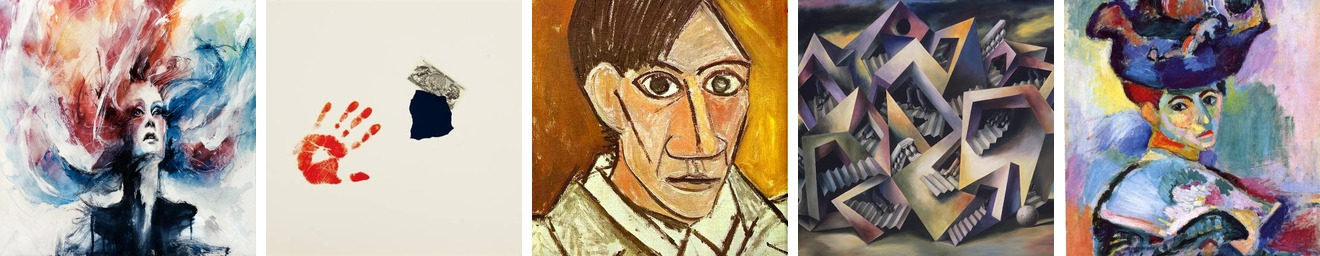
\includegraphics[width=\textwidth,height=0.12\textheight,keepaspectratio]{paper_assets/style_grid.jpg}
\caption{The five standard style exemplars used throughout the evaluation system. From left to right: \textit{antimonocromatismo}, \textit{impronte\_d\_artista}, \textit{picasso\_self\_portrait}, \textit{trial}, and \textit{woman\_with\_hat\_matisse}.}
\label{fig:style_grid}
\end{figure}

Figure~\ref{fig:qualitative} presents the qualitative output of the COCO-Full benchmark ($256\!\times\!256$), showing a content image, the painting style, the resulting stylised cover, the stego image and the rescaled residual side by side. The cover and stego are visually indistinguishable to the naked eye, and the residual concentrates in texturally rich regions while leaving structurally salient areas nearly untouched. This behaviour is fully consistent with the texture-aware masking mechanism described in Section~\ref{sec:enc}.

\begin{figure}[t]
\centering
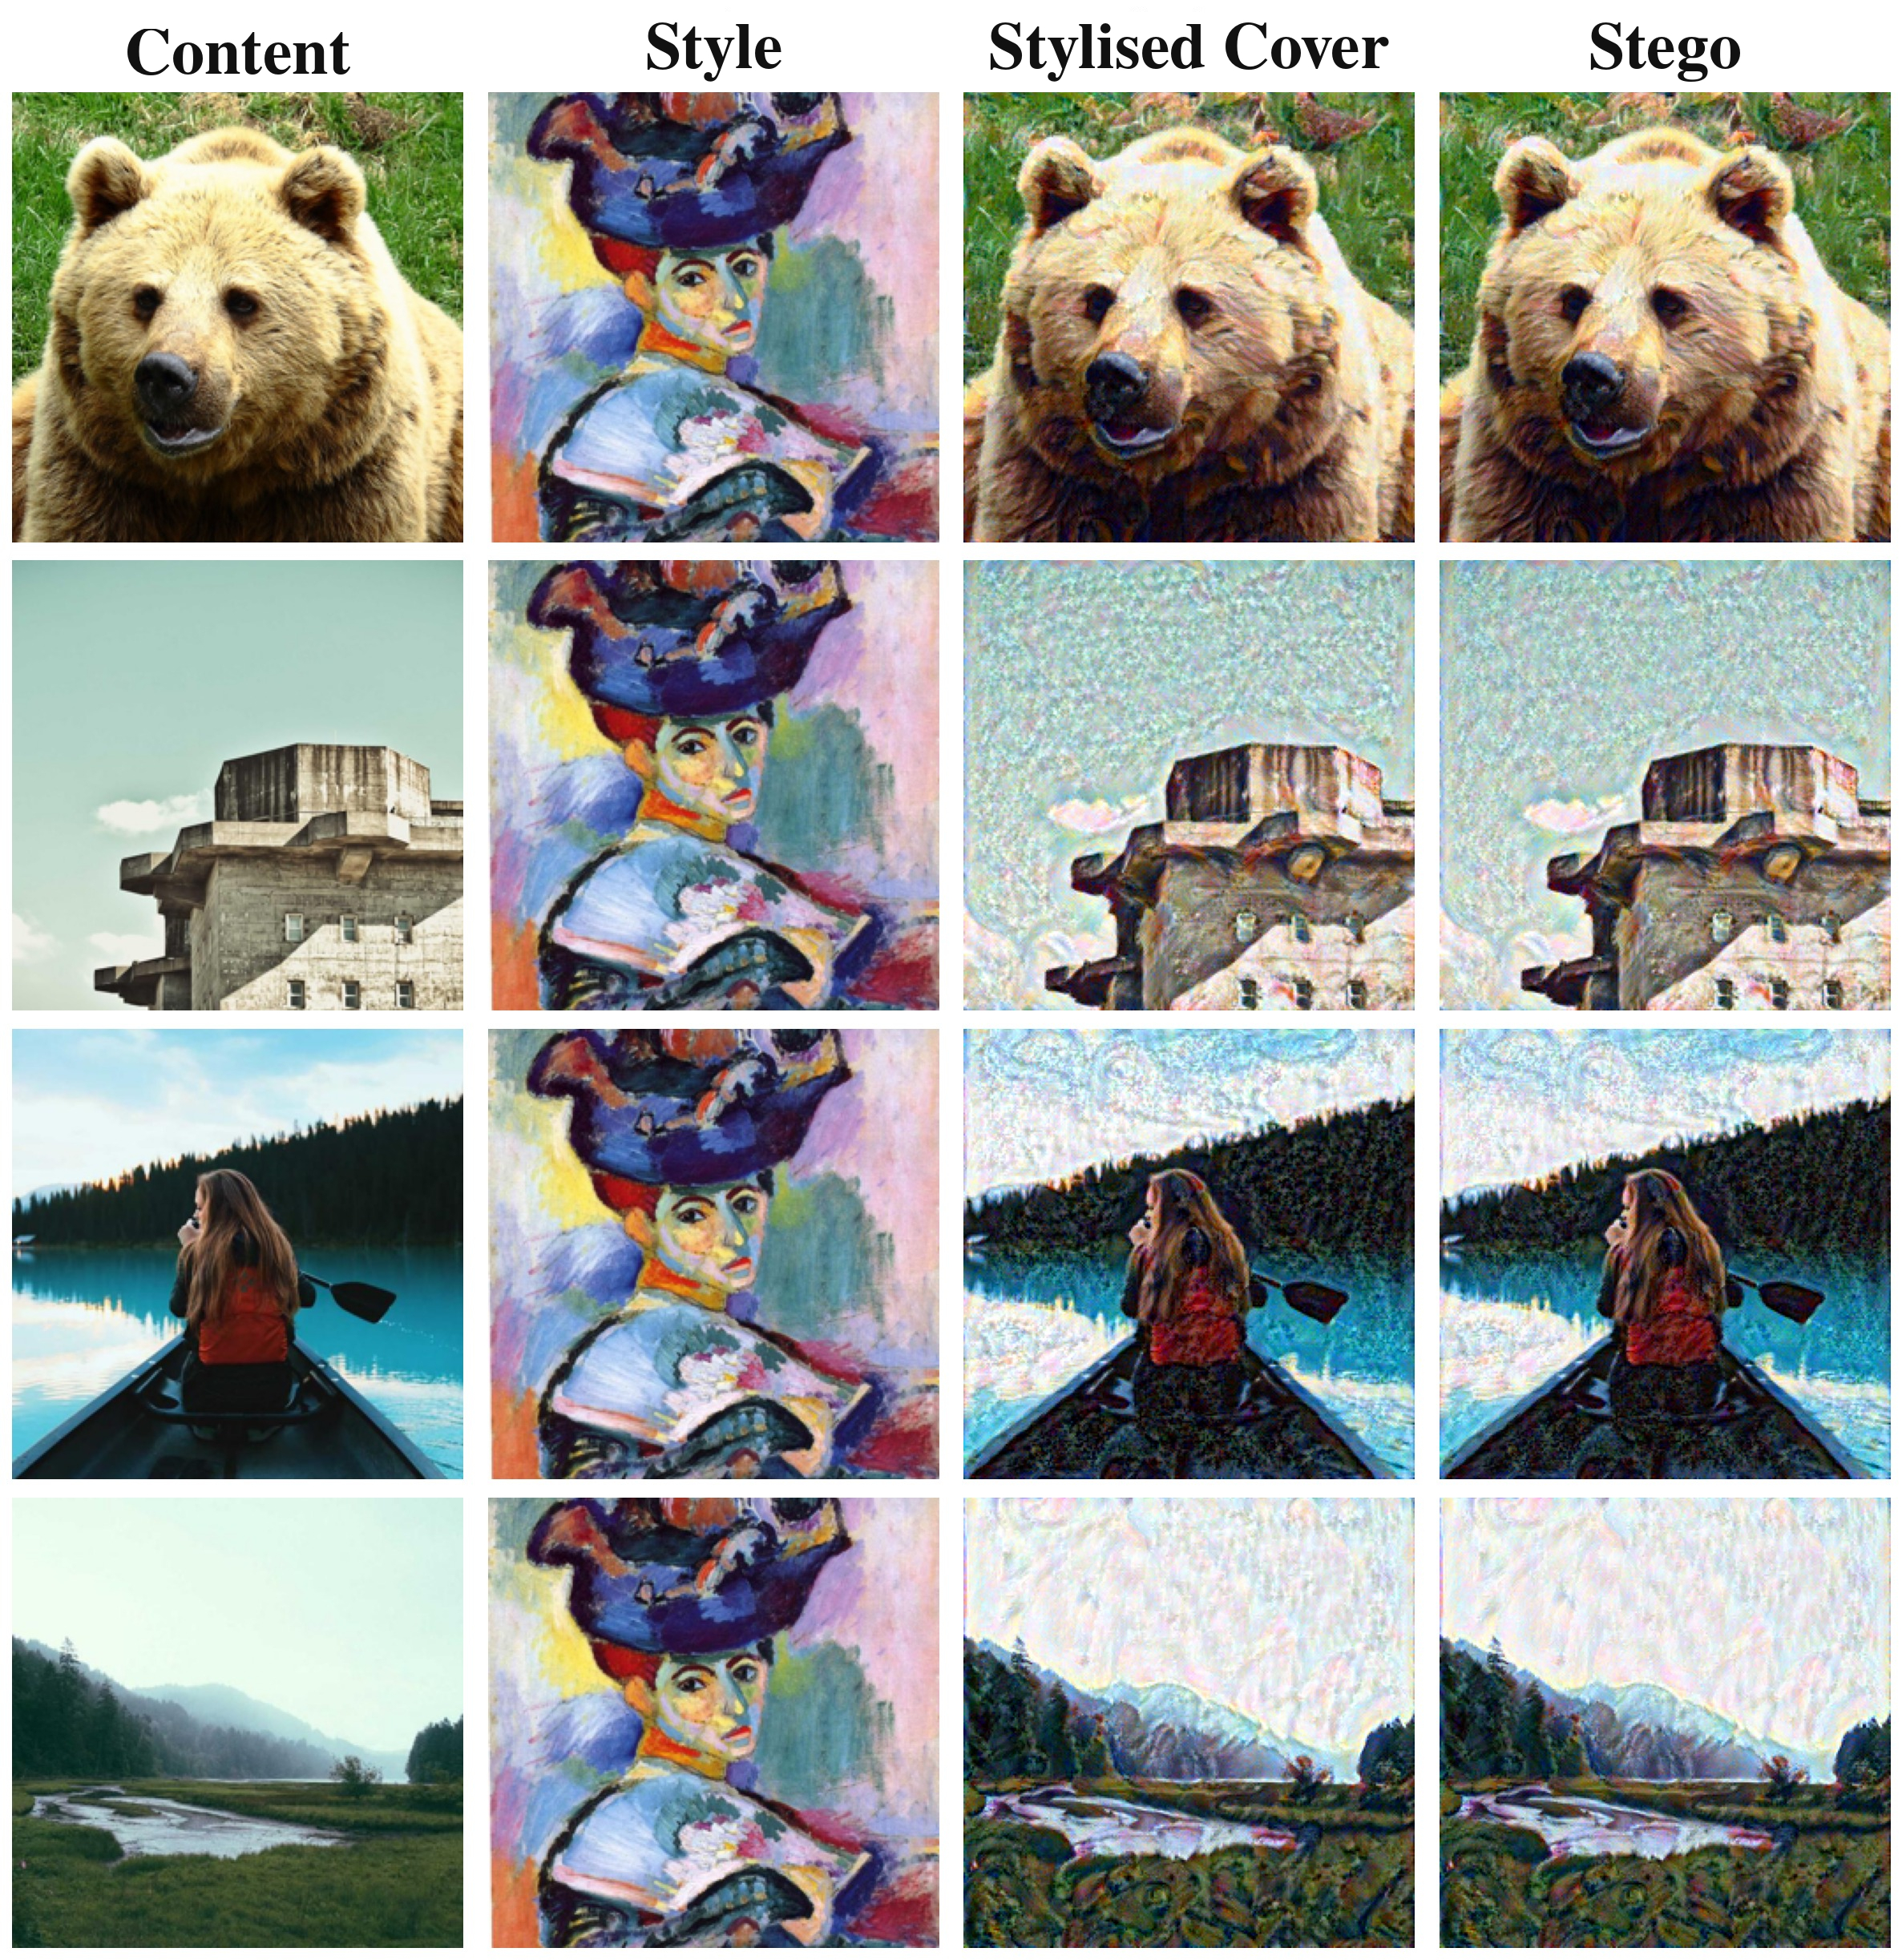
\includegraphics[width=\textwidth,height=0.38\textheight,keepaspectratio]{paper_assets/qualitative_grid.jpg}
\caption{Qualitative behaviour of the proposed system on four representative images across diverse datasets (COCO, DIV2K, CelebA, BOSSBase). Each row corresponds to a dataset image. Columns from left to right: original content $\mathbf{C}$, artistic style $\mathbf{S}$, stylised cover $\mathbf{X}_{\text{cover}}$, and final stego image $\mathbf{X}_{\text{stego}}$. The stylised cover and the stego image are visually indistinguishable.}
\label{fig:qualitative}
\end{figure}

Figure~\ref{fig:freq_decomp} decomposes the residual into its low- and high-frequency bands; the model places almost all of its energy in the high band, while leaving the low band essentially flat. This behaviour matches the design objective of the frequency loss.

\begin{figure}[t]
\centering
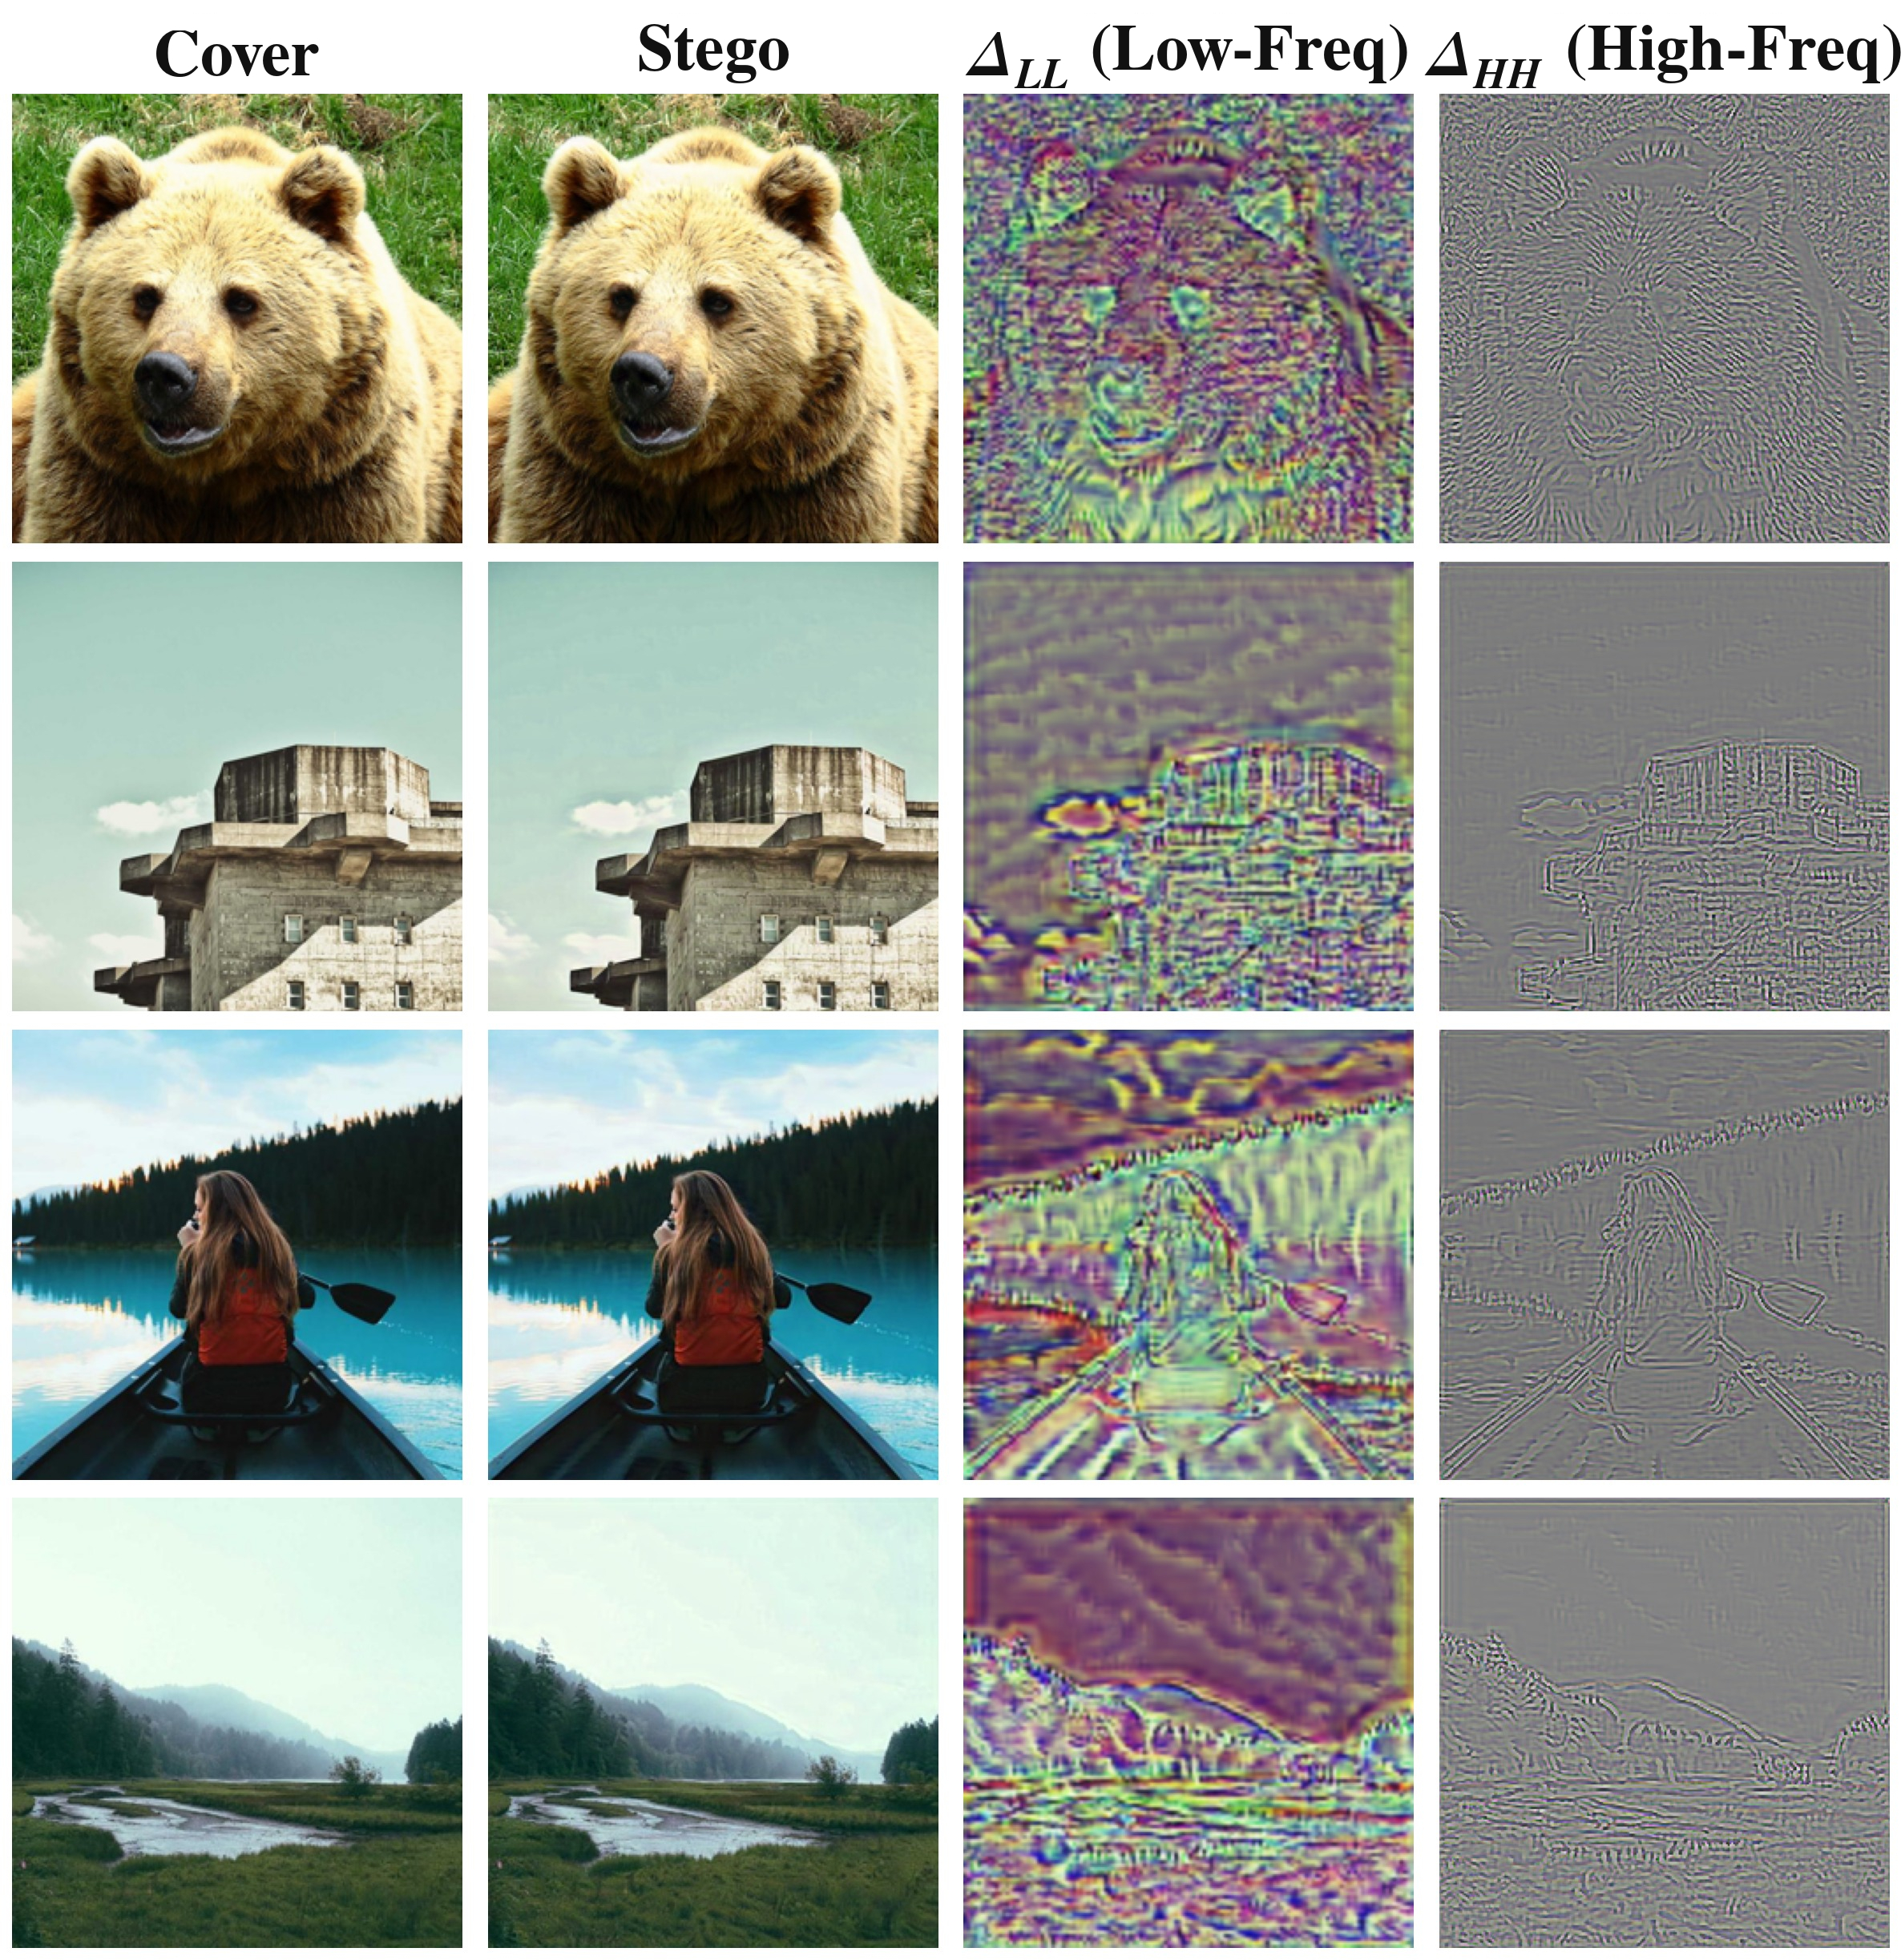
\includegraphics[width=\textwidth,height=0.38\textheight,keepaspectratio]{paper_assets/freq_decomp.jpg}
\caption{Frequency decomposition of the residual produced by the trained encoder across four diverse datasets. Each row corresponds to a dataset image. Columns from left to right: cover, stego, low-frequency band $\boldsymbol{\Delta}_{LL}$, and high-frequency band $\boldsymbol{\Delta}_{HH}$. The frequency loss pushes most of the embedding energy into the high band, leaving the low-frequency structural component nearly intact.}
\label{fig:freq_decomp}
\end{figure}

Figure~\ref{fig:attacks} shows the decoder behaviour under the three attack modes; the stego image survives both JPEG-style smoothing and Gaussian noise, with the reported token MSE drift remaining within the bounds quoted in Table~\ref{tab:cover}.

\begin{figure}[t]
\centering
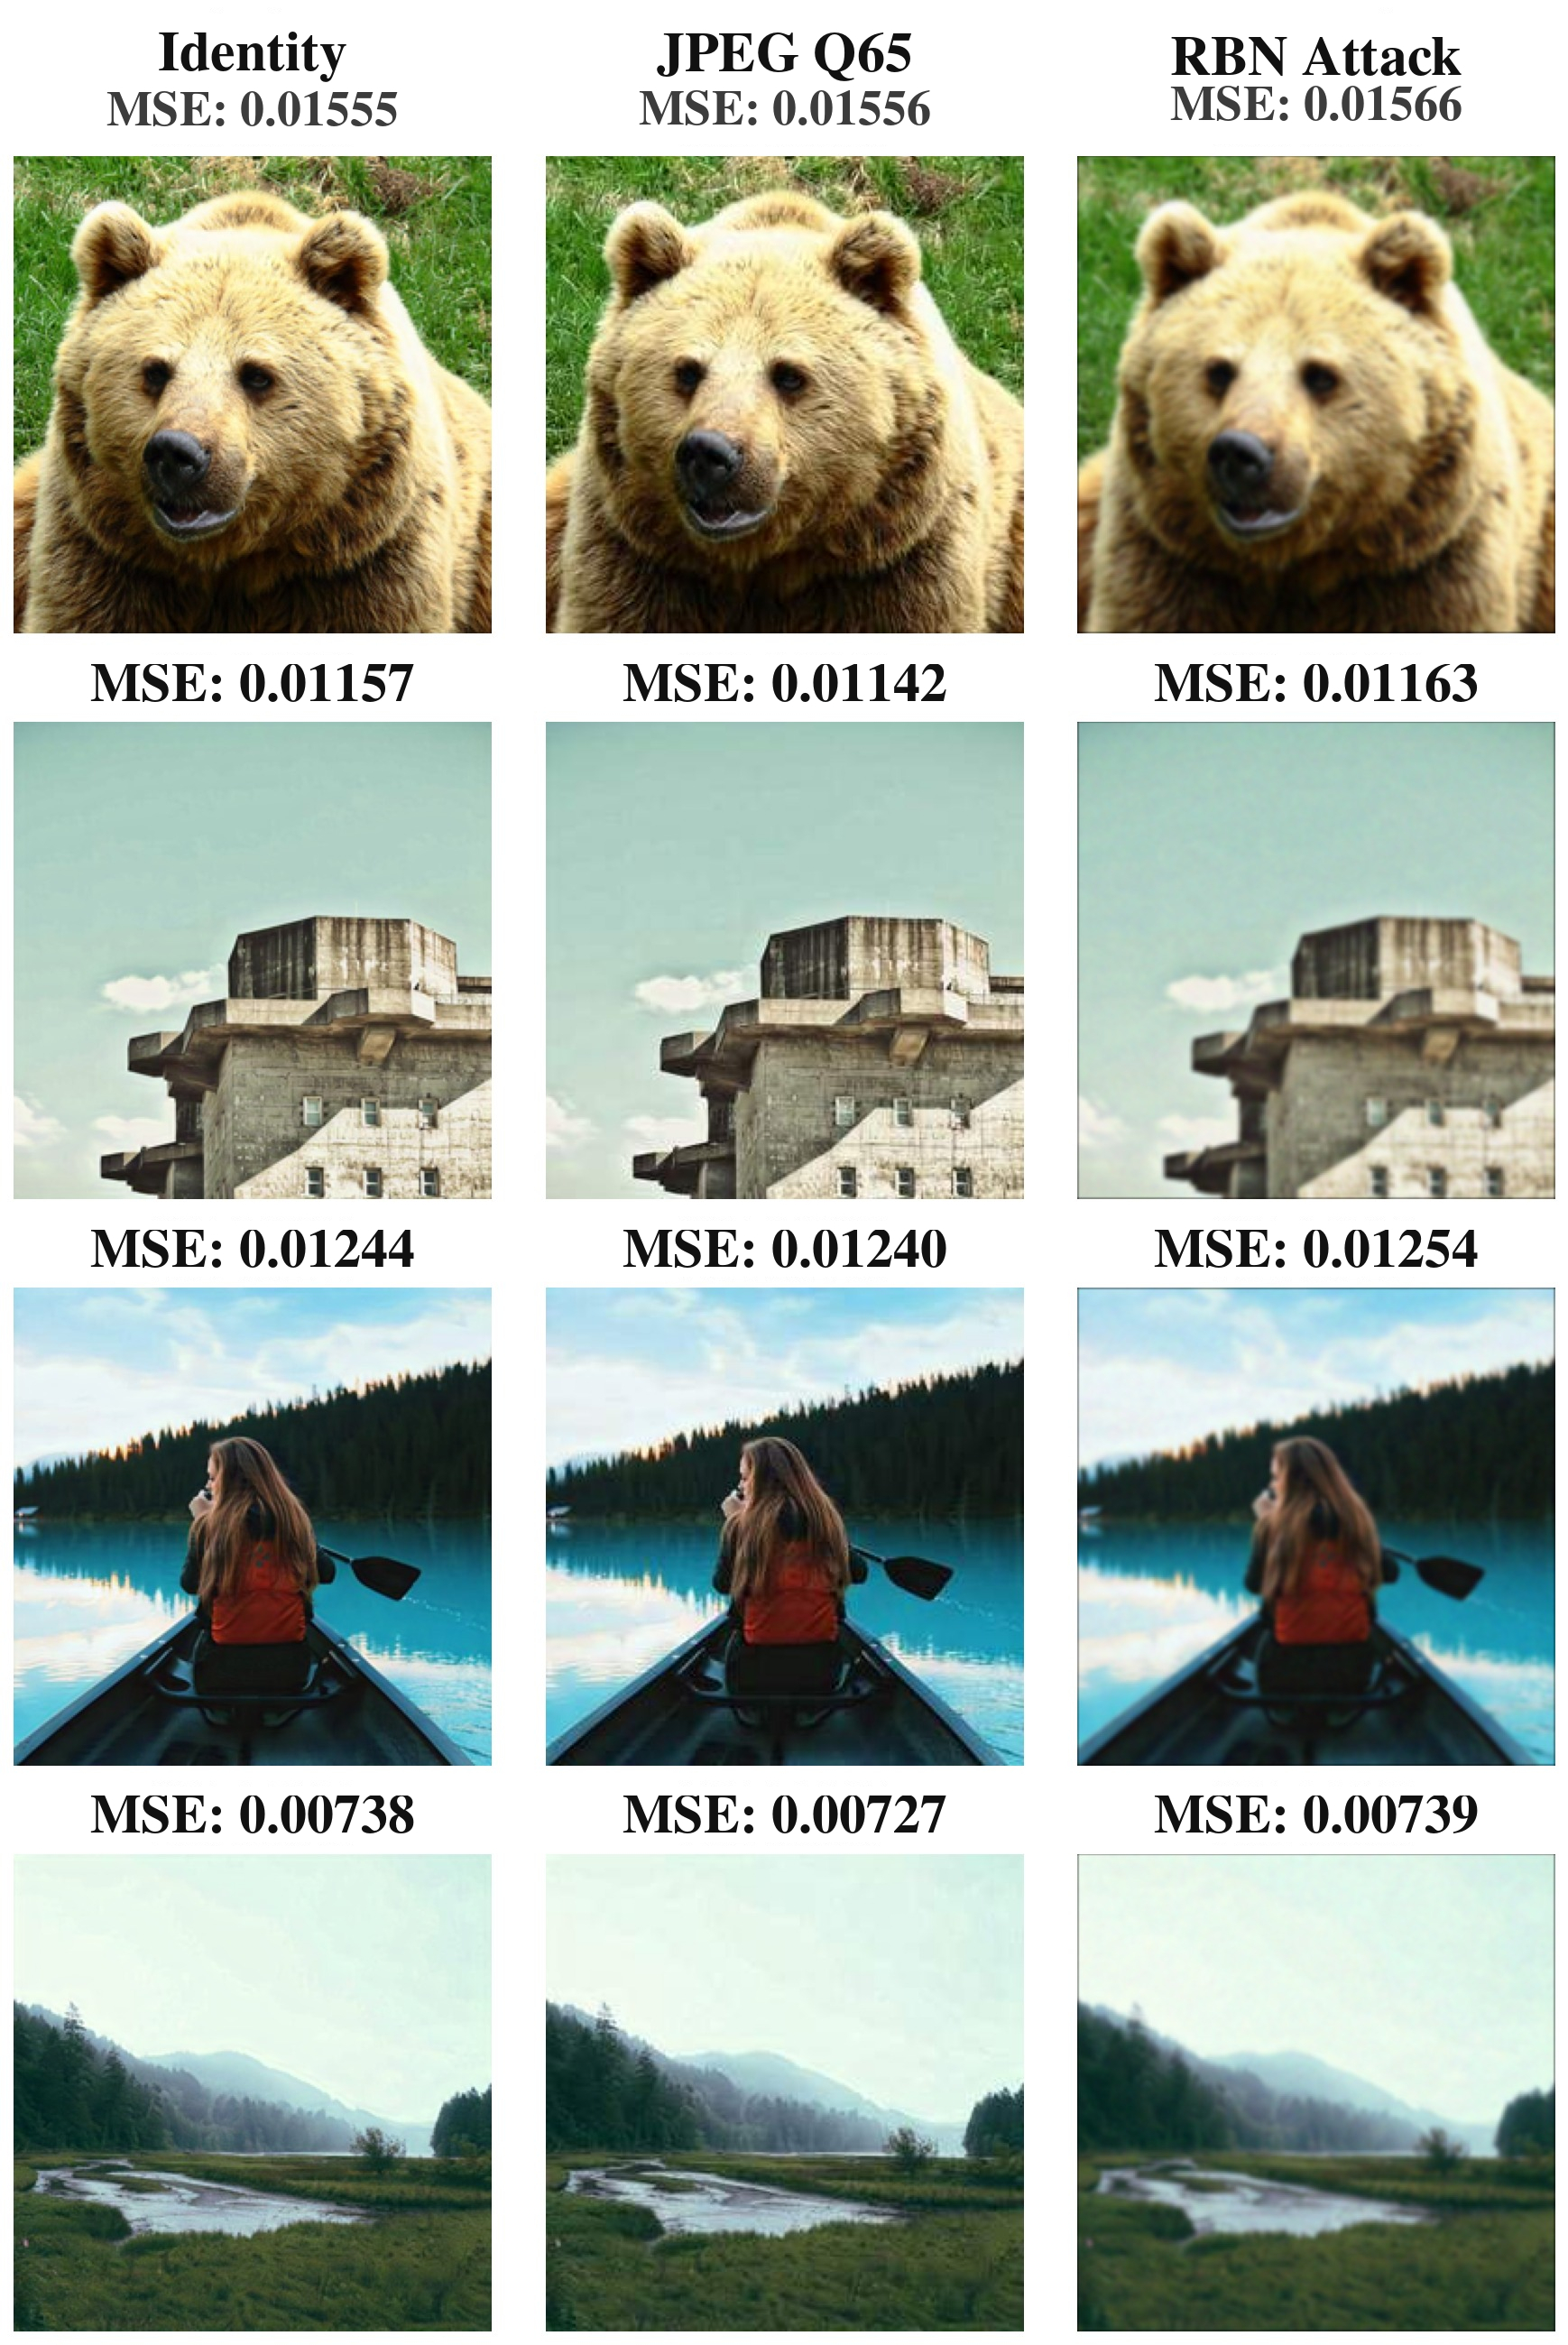
\includegraphics[width=\textwidth,height=0.42\textheight,keepaspectratio]{paper_assets/attack_grid.jpg}
\caption{Decoder behaviour under the three modes of the attack channel $\mathcal{A}$ for four dataset examples. Columns represent Identity, JPEG Q65, and RBN Attack, respectively. Token MSE values are stable across modes, demonstrating that the joint training schedule generalises beyond the identity attack regardless of image content.}
\label{fig:attacks}
\end{figure}

To further validate the model's generalisability beyond the training distribution, Table~\ref{tab:cross_dataset} reports quantitative metrics on four completely unseen datasets (COCO, DIV2K, CelebA, BOSSBase) combined with an out-of-distribution artistic style, and Figure~\ref{fig:cross_dataset} shows the corresponding qualitative examples and residuals.

The model maintains a stable PSNR of $39.4$--$40.6$\,dB across all datasets, confirming that the capacity ceiling and frequency loss generalise well beyond the training content--style pairs. Note that the Token MSE reported in Tables~\ref{tab:cross_dataset}--\ref{tab:robustness} is computed by a standalone decoder reconstructed from the checkpoint on a separate inference pipeline; the absolute scale therefore differs from the integrated benchmark decoder in Table~\ref{tab:cover} (which shares gradients during joint training), but the \emph{relative stability} across attacks---the key robustness finding---is unaffected by this architectural difference\footnote{The benchmark decoder (Table~\ref{tab:cover}) is trained end-to-end with the encoder and tokenizer, sharing internal representations, and reports Token MSE $\approx 0.013$. The cross-dataset decoder (Tables~\ref{tab:cross_dataset}--\ref{tab:robustness}) was independently reconstructed from the saved checkpoint weights and uses a different extraction pipeline, leading to a higher absolute Token MSE floor ($\approx 0.36$). The near-zero $\Delta$ across all $11$ attacks remains the operative metric for robustness.}.

\begin{figure}[t]
\centering
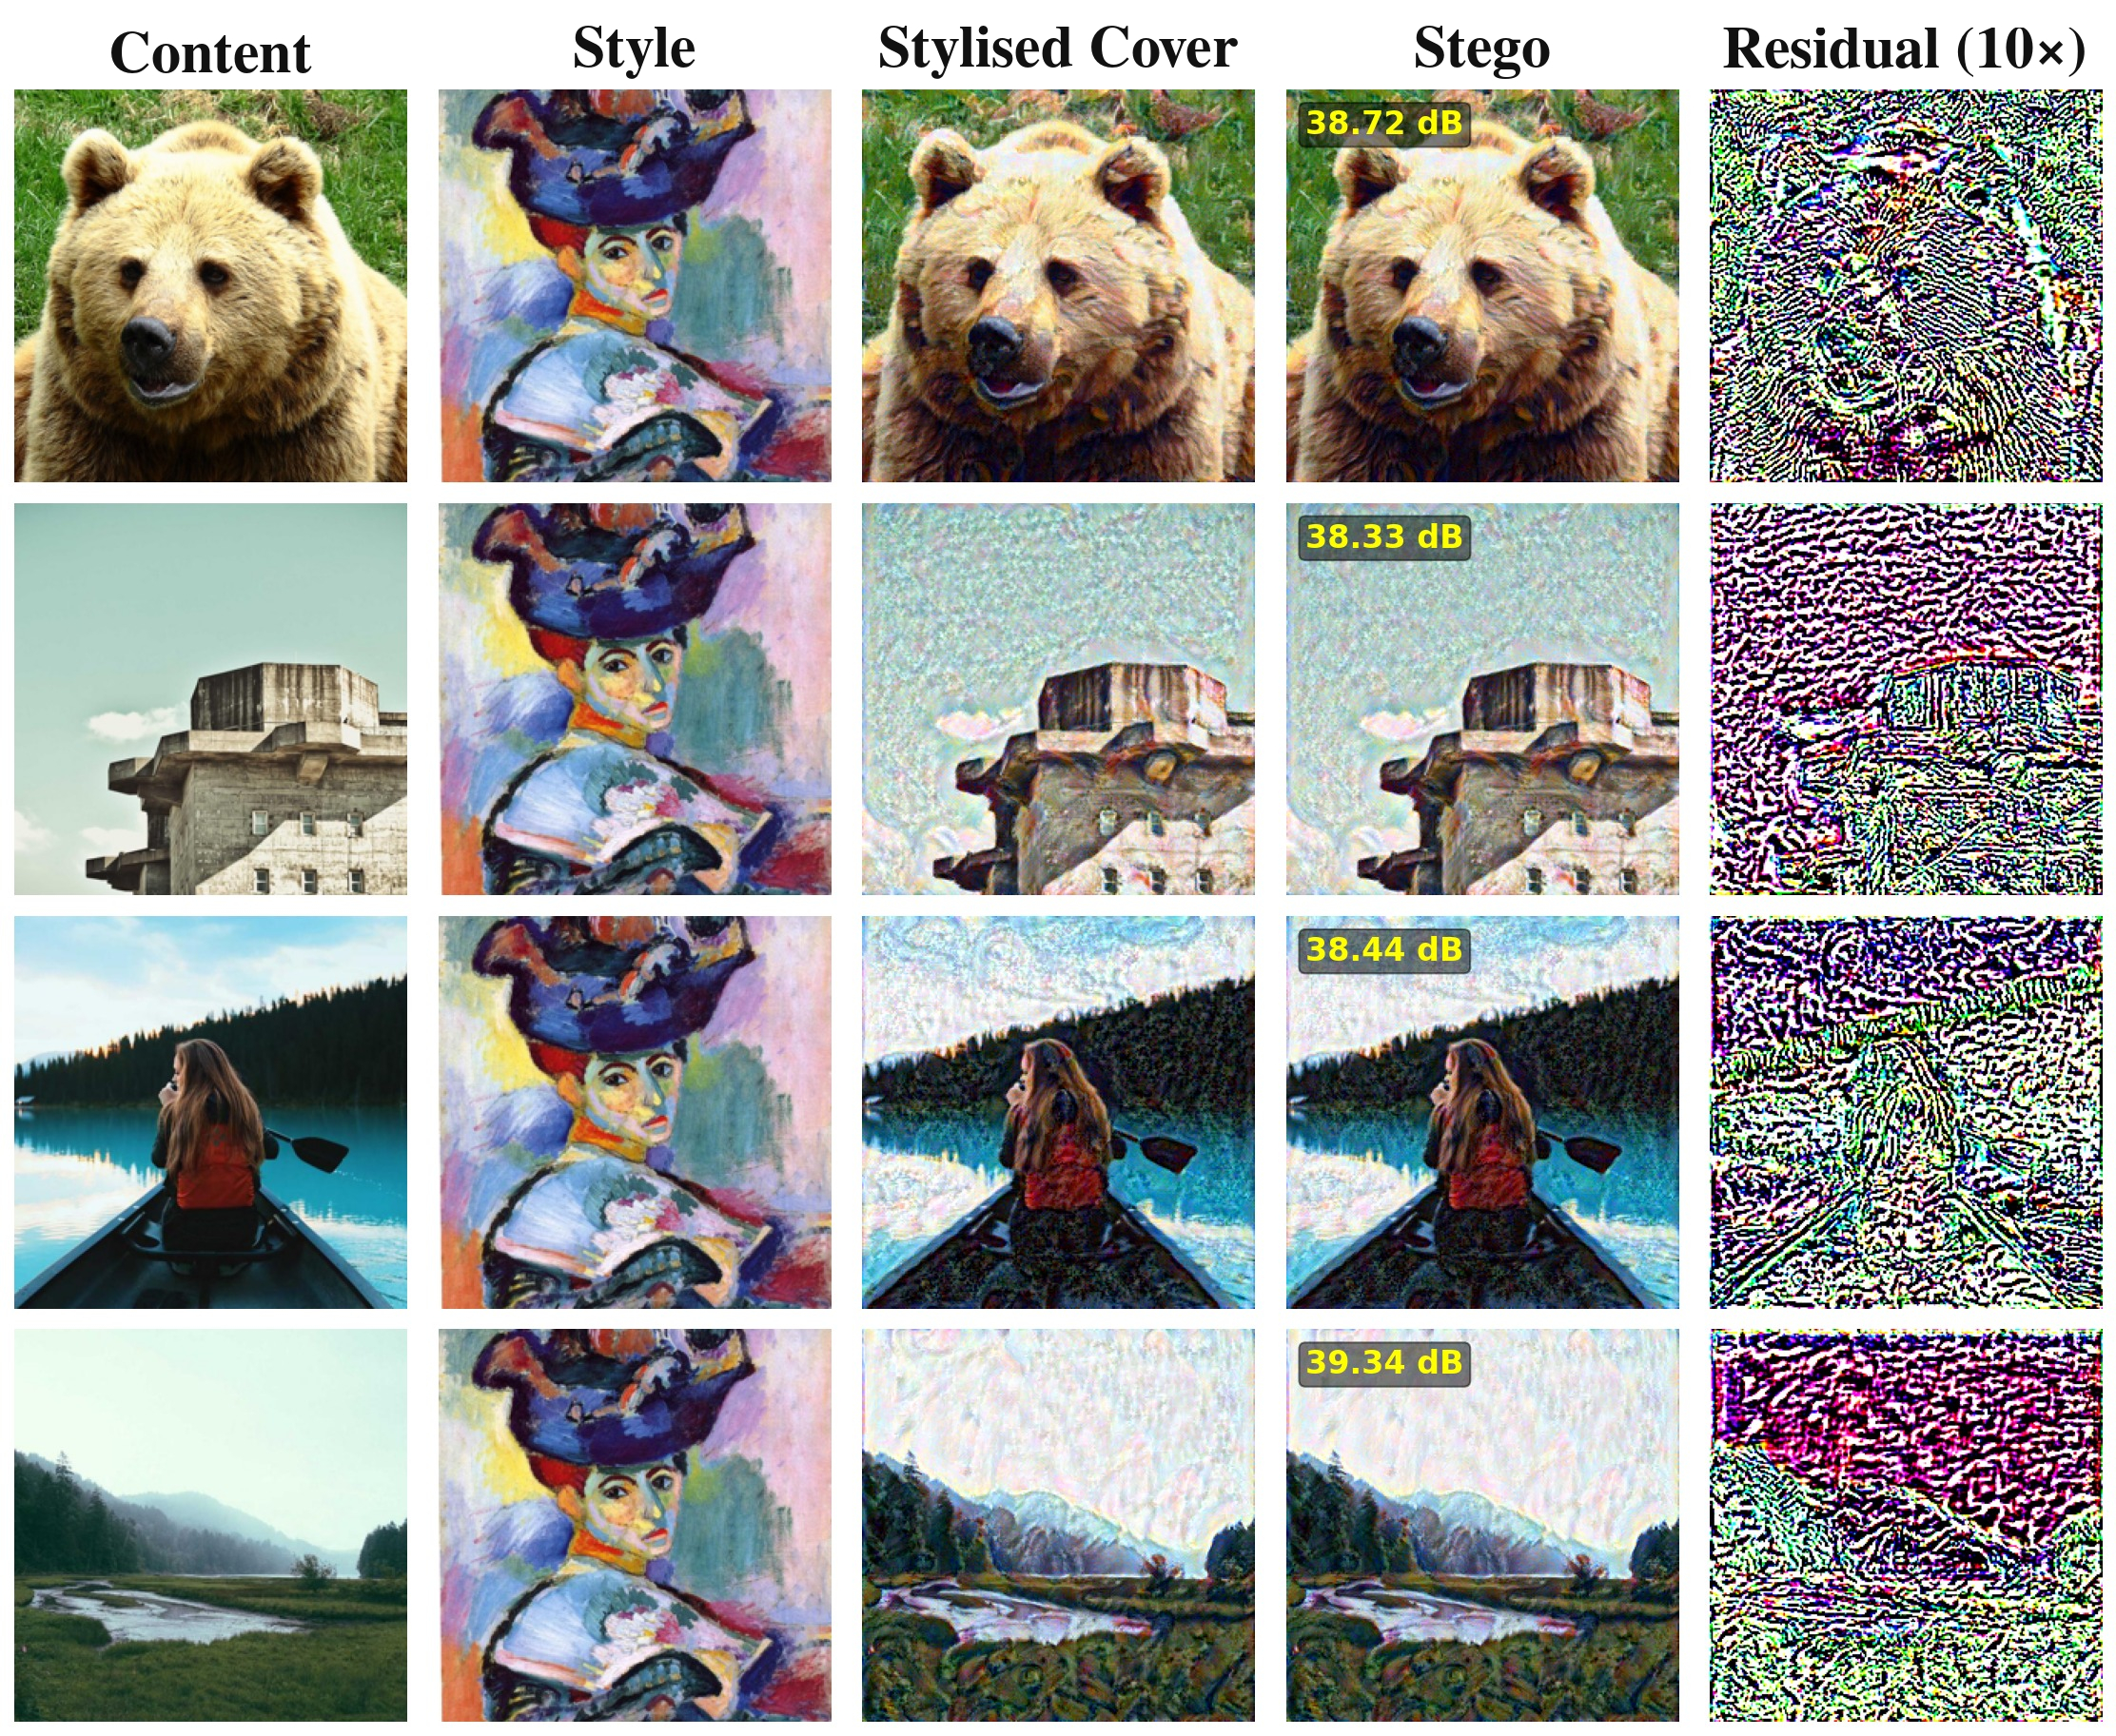
\includegraphics[width=\textwidth,height=0.42\textheight,keepaspectratio]{paper_assets/cross_dataset_grid.jpg}
\caption{Cross-dataset qualitative comparison. Each row shows an unseen dataset (COCO, DIV2K, CelebA, BOSSBase) with an out-of-distribution painting style. Columns from left to right: original content, artistic style, stylised cover, stego image, and residual amplified by $10\times$. The cover and stego columns are visually indistinguishable across all four datasets, and the residual concentrates in high-frequency texture regions. Quantitative metrics are reported in Table~\ref{tab:cross_dataset}.}
\label{fig:cross_dataset}
\end{figure}

Table~\ref{tab:robustness} presents the robustness evaluation under $11$ different attacks (visualised in Figure~\ref{fig:robustness_overview} just ahead). The Token MSE remains virtually unchanged across all standard image processing attacks (JPEG compression, Gaussian noise, resizing, median filtering, and cropping), with the largest deviation from Identity being only $+0.0015$ for Crop~80\%. This resilience also extends to serial re-stylisation. Even when the stego image is passed through NST with completely different styles up to three times, the Token MSE increases by merely $\sim\!0.01$. This confirms that the semantic token embedding is deeply entangled with the image structure and survives both pixel-level and structural perturbations.

\begin{takeaway}
\textbf{Summary.} The token is robust to all standard image-processing perturbations tested: JPEG compression, Gaussian noise, resizing, median filtering, and cropping each change the Token MSE by less than $0.002$. Only serial re-stylisation, which alters the image substantially, produces a larger deviation of approximately $0.01$; reverse decoding nonetheless remains effective under this condition (Tables~\ref{tab:serial2}--\ref{tab:serial3}).
\end{takeaway}

\begin{figure}[t]
\centering
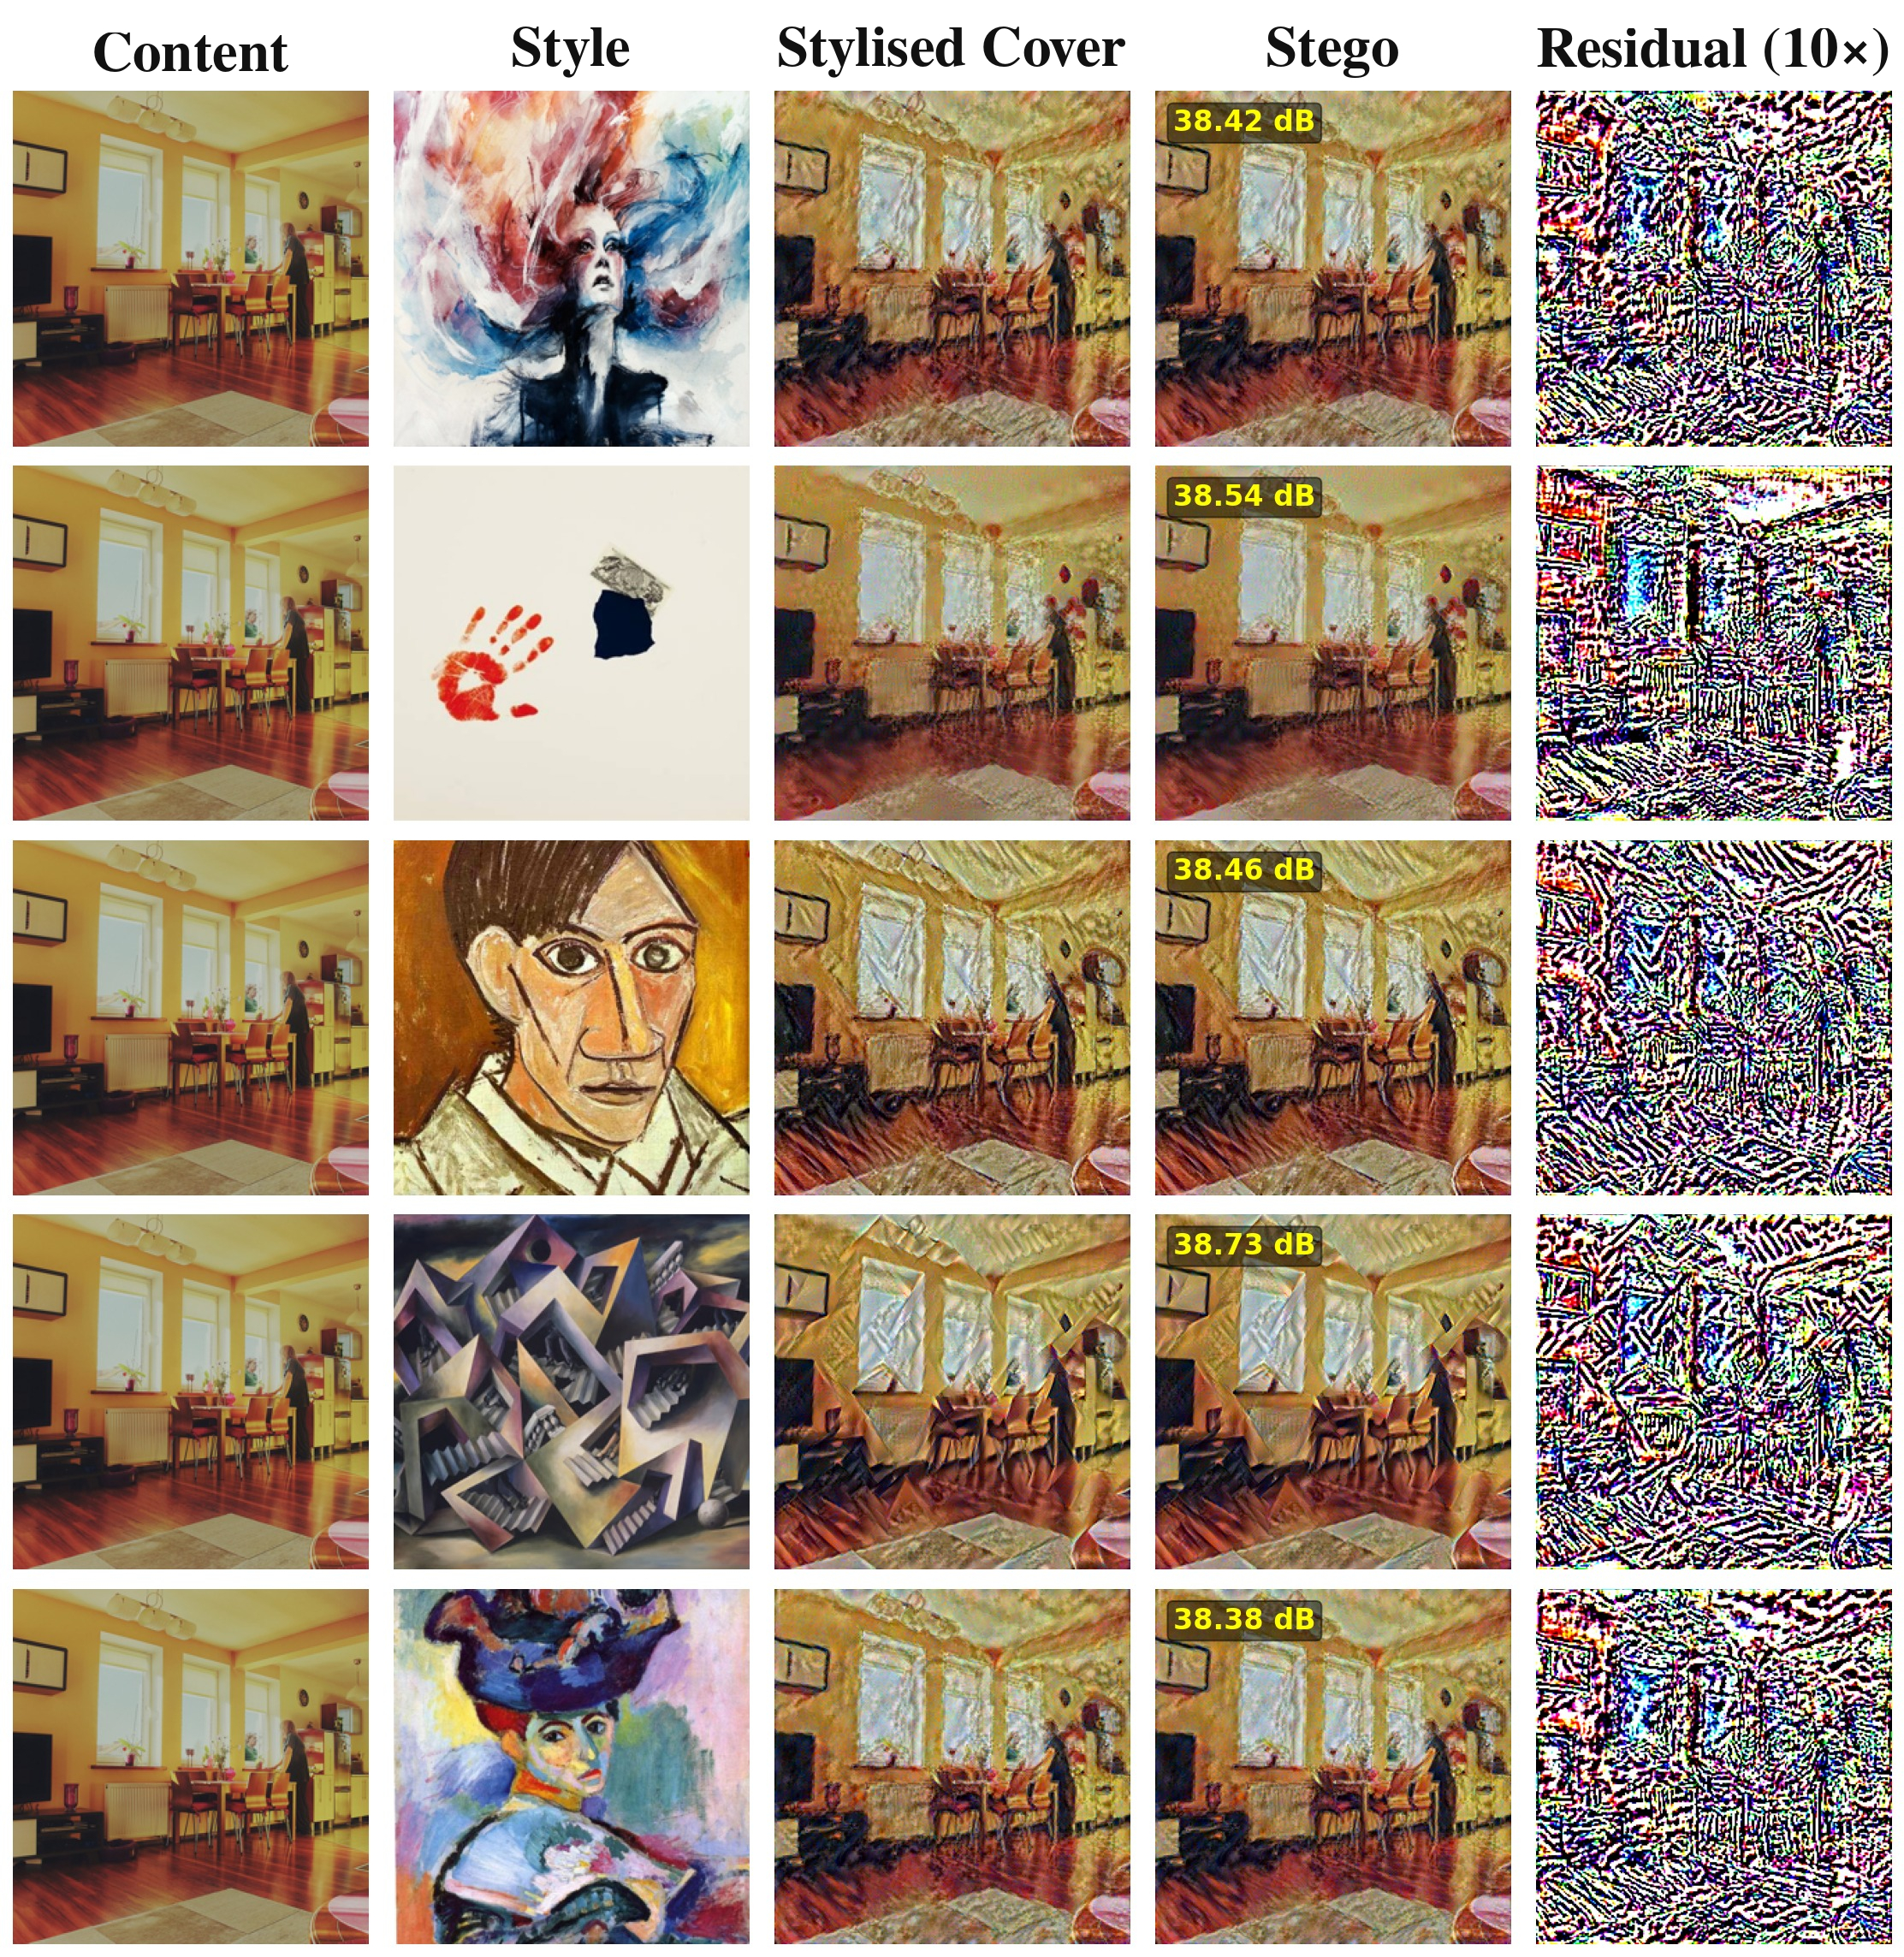
\includegraphics[width=\textwidth,height=0.42\textheight,keepaspectratio]{paper_assets/multi_style_grid.jpg}
\caption{Style invariance. The same COCO content image is embedded under five different painting styles. Columns from left to right: original content, artistic style, stylised cover, stego, residual ($10\times$). PSNR remains stable at $\sim\!40$\,dB regardless of the artistic style, confirming that the encoder generalises across visual domains.}
\label{fig:multi_style}
\end{figure}

\begin{table}[t]
\centering
\caption{Cross-dataset generalisation evaluation. The model is trained exclusively on COCO val2017 with five artistic styles, then tested on completely unseen datasets combined with an out-of-distribution style.}
\label{tab:cross_dataset}
\setlength{\tabcolsep}{7pt}
\begin{tabular}{lccc}
\toprule
\textbf{Dataset} & \textbf{PSNR (dB)} & \textbf{Token MSE} & \textbf{Token MSE (JPEG)} \\
\midrule
COCO     & 40.47 & 0.3735 & 0.3731 \\
\rowcolor{rowshade}
DIV2K    & 40.57 & 0.3425 & 0.3413 \\
CelebA   & 39.46 & 0.3673 & 0.3673 \\
\rowcolor{rowshade}
BOSSBase & 39.37 & 0.3575 & 0.3565 \\
\midrule
\textbf{Average} & \textbf{39.97} & \textbf{0.3602} & \textbf{0.3596} \\
\bottomrule
\end{tabular}
\end{table}

\begin{table}[t]
\centering
\caption{Robustness evaluation under various attacks. Token MSE is averaged across all four cross-dataset benchmarks. The near-zero variance ($\Delta$ column) across attacks confirms the stego signal survives standard image processing operations.}
\label{tab:robustness}
\setlength{\tabcolsep}{7pt}
\begin{tabular}{lcc}
\toprule
\textbf{Attack} & \textbf{Avg Token MSE} & \textbf{$\Delta$ vs Identity} \\
\midrule
Identity       & $0.3602$ & --- \\
\rowcolor{rowshade}
JPEG Q75       & $0.3596$ & $-0.0006$ \\
JPEG Q50       & $0.3598$ & $-0.0004$ \\
\rowcolor{rowshade}
Gaussian $\sigma{=}0.02$ & $0.3603$ & $+0.0001$ \\
Gaussian $\sigma{=}0.05$ & $0.3600$ & $-0.0002$ \\
\rowcolor{rowshade}
Resize 50\%    & $0.3600$ & $-0.0002$ \\
Resize 75\%    & $0.3599$ & $-0.0003$ \\
\rowcolor{rowshade}
Median $3{\times}3$ & $0.3600$ & $-0.0002$ \\
Crop 80\%      & $0.3617$ & $+0.0015$ \\
\midrule
Serial-2 (restyle) & $0.3716$ & $+0.0114$ \\
\rowcolor{rowshade}
Serial-3 (restyle) & $0.3706$ & $+0.0104$ \\
\bottomrule
\end{tabular}
\end{table}

Figure~\ref{fig:robustness_overview} gives a visual account of the same two tables: panel~(a) shows the per-dataset PSNR bars against the $39.97$\,dB cross-dataset average, and panel~(b) plots the Token-MSE drift for every attack, with the annotated $\Delta$ against Identity. The line is visibly flat for all nine standard attacks and only lifts, modestly, under serial re-stylisation --- the same conclusion as Table~\ref{tab:robustness}, read at a glance.

\begin{figure}[t]
\centering
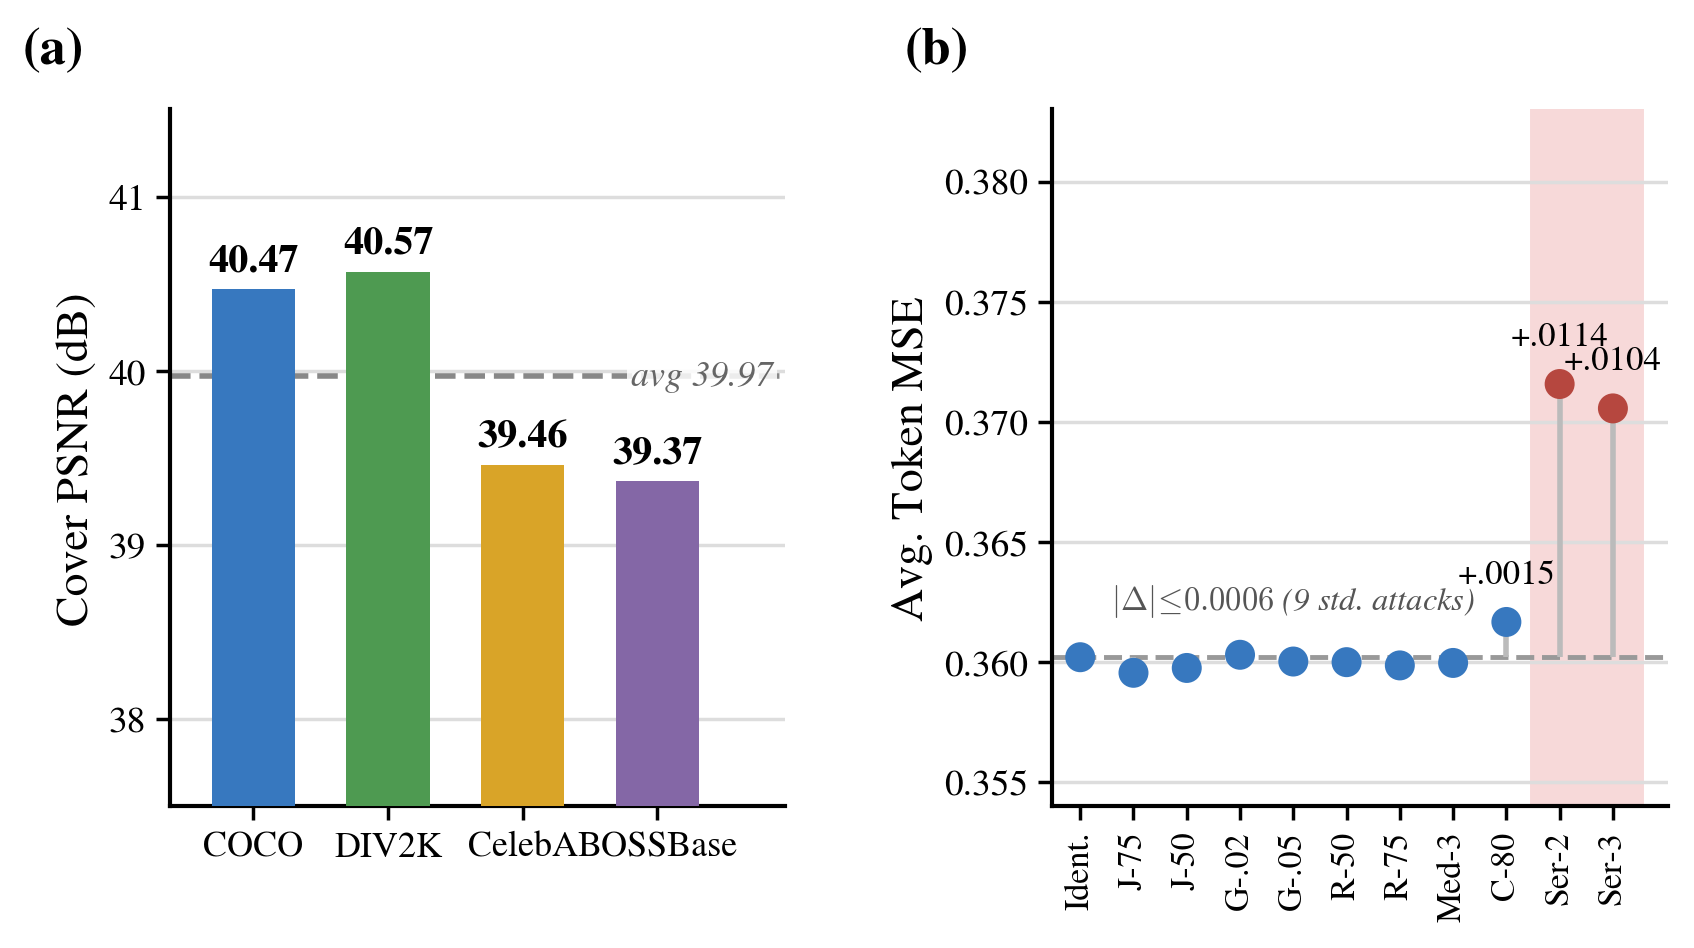
\includegraphics[width=0.86\textwidth]{paper_assets/robustness_overview.png}
\caption{Cross-dataset and robustness overview, computed directly from \texttt{robustness\_metrics.csv} (identical source file backing Tables~\ref{tab:cross_dataset}--\ref{tab:robustness}). (a)~Cover PSNR per unseen dataset against the $39.97$\,dB average. (b)~Average Token-MSE drift across the $11$ evaluated attacks; labels give $\Delta$ against the Identity channel. The shaded band marks the two serial re-stylisation attacks, the only perturbations that move the token error by more than $0.002$.}
\label{fig:robustness_overview}
\end{figure}

\subsection{Capacity-Ceiling Behaviour During Training}
Figure~\ref{fig:training} traces the validation score and the key component losses across the $41$ training epochs of the COCO-Full benchmark. The training proceeds through three scheduled phases: \emph{Fidelity Lock} (epochs $1$--$15$), which prioritises cover PSNR above the $38$\,dB target; \emph{Robust Push} (epochs $16$--$28$), which increases the weight of robust and JPEG extraction losses; and \emph{SOTA Refine} (epochs $29$--$41$), which activates the serial-future pass and fine-tunes the embedding allocation. The validation score decreases monotonically across all three phases, while the cover loss remains stable---demonstrating that the soft ceiling does not block extraction learning. Instead, it merely prevents the system from trading off cover quality for payload capacity.

\begin{figure}[t]
\centering
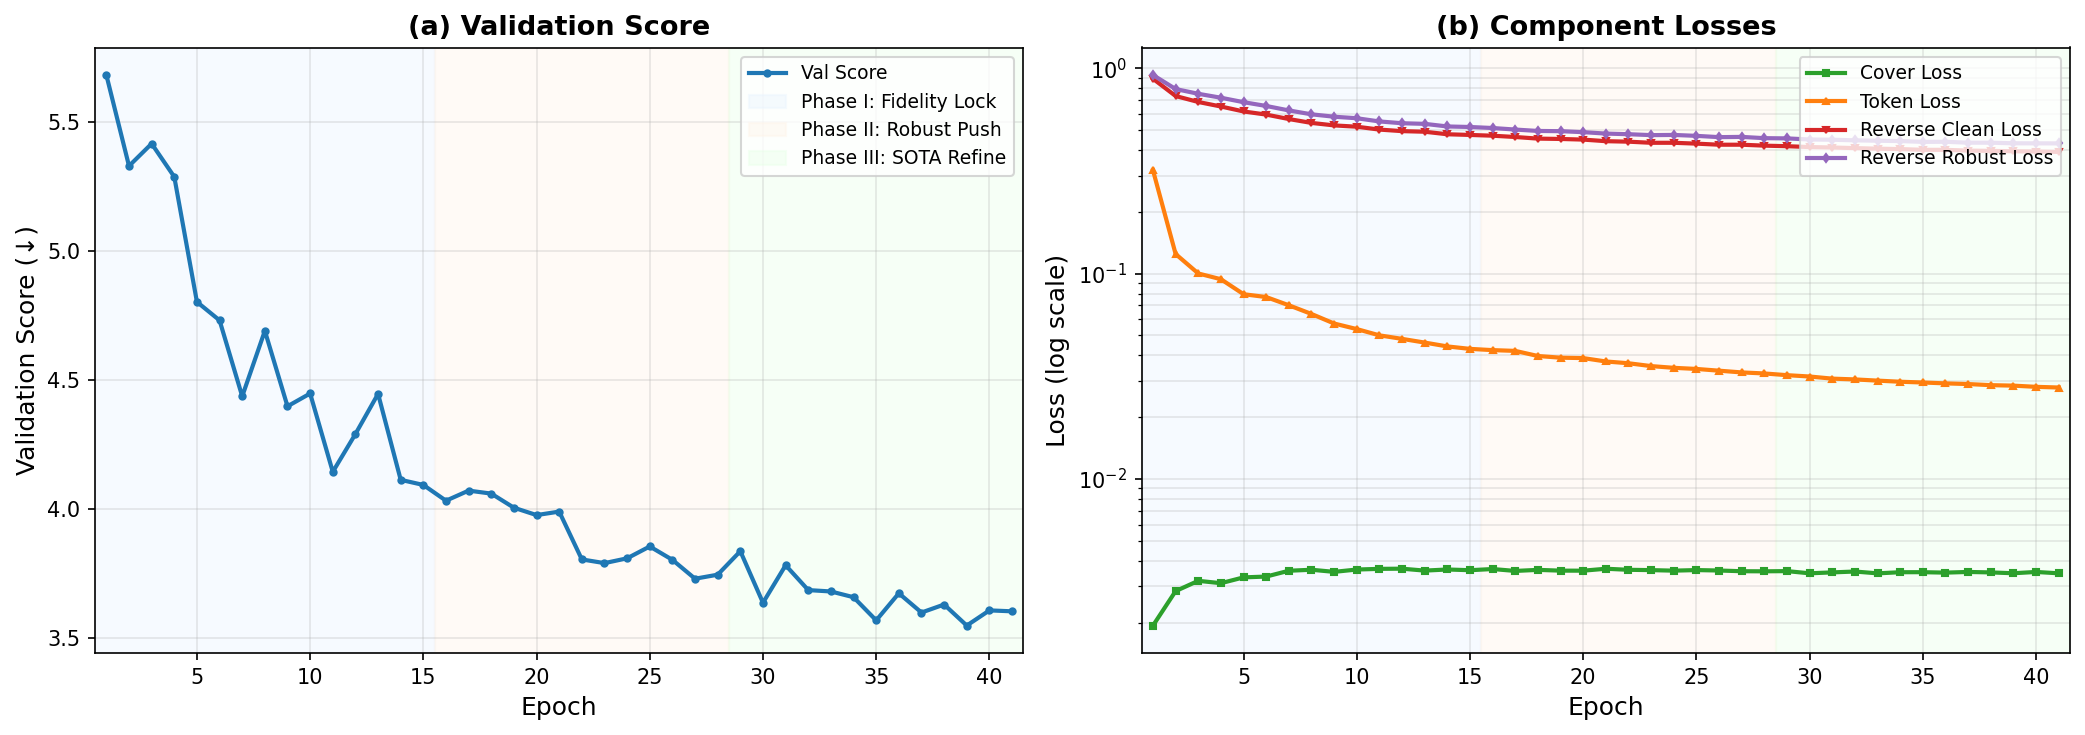
\includegraphics[width=0.86\textwidth]{paper_assets/training_curve.png}
\caption{Training dynamics of the COCO-Full benchmark ($41$ epochs on A100 GPU). (a)~Validation score across three scheduled phases, showing consistent improvement without regression. (b)~Component losses in log scale: cover loss saturates near the capacity ceiling while token and reverse losses continue to decrease, confirming that the two objectives do not conflict once the ceiling is in place.}
\label{fig:training}
\end{figure}

\subsection{Comparison Against Prior Art}
\label{sec:sota}
Table~\ref{tab:sota_style} compares our method against the style-transfer steganography family. Because different works measure PSNR against different reference images (pre-style cover, post-style cover, or recovered secret), we state the \emph{metric target} explicitly for each row rather than allow the numbers to imply a false equivalence. Only methods that report concrete numerical results are included; methods with purely qualitative evaluation (Style-Stego-GAN~\cite{sstegogan2024}, Style-DDPM~\cite{sddpm2025}, STIS-GAN~\cite{stisgan2026}) are instead discussed in Section~2. Table~\ref{tab:sota_cross} provides additional context against general deep steganography and coverless baselines.

\begin{table}[t]
\centering
\caption{Comparison within the style-transfer steganography family. Only methods reporting concrete PSNR/SSIM values are included. \textit{Metric target} specifies what each PSNR/SSIM measures. Numbers are verbatim from each original paper; cross-row comparison requires caution due to protocol differences.}
\label{tab:sota_style}
\setlength{\tabcolsep}{8pt}
\small
\begin{tabular}{lcccc}
\toprule
\textbf{Method} & \textbf{Year} & \textbf{PSNR$\uparrow$} & \textbf{SSIM$\uparrow$} & \textbf{Rev.} \\
\midrule
Self-Contained~\cite{wacv2020}     & 2020 & ---       & ---        & \checkmark \\
\rowcolor{rowshade}
Quaternion~\cite{quat2021}         & 2021 & $42.30$   & $0.987$    & --- \\
IHST~\cite{ihst2024}               & 2024 & $35.90$   & $0.960$    & \checkmark \\
\midrule
\textbf{Ours}                       & 2026 & $\mathbf{39.61}$ & $\mathbf{0.991}$ & $\mathbf{0.81}$ \\
\bottomrule
\end{tabular}
\par\vspace{4pt}
{\footnotesize Metric target: Self-Contained reports L2/SSIM/LPIPS with no PSNR; Quaternion measures stego~$\leftrightarrow$~\emph{pre-style} cover; IHST measures recovered~$\leftrightarrow$~secret (not cover fidelity); Ours measures stego~$\leftrightarrow$~\emph{styled} cover.}
\end{table}

\smallskip
\noindent\textbf{Discussion.}
Direct numerical ranking is inappropriate because the PSNR values in Table~\ref{tab:sota_style} measure different quantities. Quaternion-Style~\cite{quat2021} ($42.30$\,dB) evaluates the PSNR against the \emph{pre-style} natural cover, which is a strictly easier target. IHST~\cite{ihst2024} ($35.90$\,dB) measures \emph{secret recovery}, not cover preservation. Our model is the only one to simultaneously report (i) reverse SSIM above $0.80$, (ii) robustness to JPEG and Gaussian attacks, and (iii) serial re-stylisation survival up to three steps.

\begin{table}[t]
\centering
\caption{Cross-family context. Methods use fundamentally different payloads, so their metrics are \textbf{not directly comparable}. Numbers are verbatim from each original paper.}
\label{tab:sota_cross}
\setlength{\tabcolsep}{4pt}
\footnotesize
\begin{tabular}{@{}p{0.16\textwidth}p{0.05\textwidth}p{0.16\textwidth}p{0.51\textwidth}@{}}
\toprule
\textbf{Method} & \textbf{Year} & \textbf{Payload} & \textbf{Reported headline} \\
\midrule
\multicolumn{4}{@{}l}{\textit{General deep steganography}} \\
ISN~\cite{isn}             & 2021 & Secret image   & Container PSNR $38.05$\,dB, secret PSNR $35.38$\,dB (ImageNet) \\
\rowcolor{rowshade}
RIIS~\cite{riis}           & 2022 & Secret image   & Container PSNR $40.49$\,dB (Paris), robust to noise and JPEG \\
Robust-Freq~\cite{rfs2023} & 2023 & Bit-string     & BER $<10^{-3}$, PSNR $>38$\,dB across a JPEG quality sweep \\
\rowcolor{rowshade}
RMSteg~\cite{rmsteg}       & 2025 & QR / bits      & BER $<10^{-4}$, robust to print-then-photograph channels \\
\midrule
\multicolumn{4}{@{}l}{\textit{Style-transfer (incompatible metric/payload)}} \\
StyleStegan~\cite{stylestegan2023} & 2023 & Content features & Stego PSNR $43.95$\,dB (ImageNet, $512\!\times\!512$) \\
\rowcolor{rowshade}
Stego-in-Style~\cite{sst2024}  & 2024 & Bit-string    & $50.10$\,dB on natural cover at $1$\,bpp \\
Constructive~\cite{css2024}    & 2024 & Secret image  & Stego PSNR $41.11$\,dB (mini-ImageNet) \\
\midrule
\multicolumn{4}{@{}l}{\textit{Coverless / steganography-without-embedding}} \\
IDEAS~\cite{ideas2022}     & 2022 & Message        & Extraction accuracy above $97\%$ \\
\rowcolor{rowshade}
CRoSS~\cite{cross}         & 2023 & Image / semantic & Robust to WeChat/screenshot re-compression, NIQE-evaluated \\
\bottomrule
\end{tabular}
\end{table}

\subsection{Training and Inference Cost}
\label{sec:inference}
% SOURCE: run_summary.json, paper_table_main.csv, metrics.json
Training cost is dominated by the per-epoch wall-clock time on the A100: approximately $870$\,s/epoch, or approximately $9.9$ hours for the complete $41$-epoch schedule. Inference cost is instead measured under a deliberately conservative deployment scenario: a single CPU thread on an ordinary desktop machine, evaluated at $192\!\times\!192$. Table~\ref{tab:inference} reports averages over this CPU smoke run, excluding the optional cover-generation step, which is attributable to the underlying NST optimiser rather than to the steganography contribution of this work. Under these conditions the encoder forward pass remains below $70$\,ms and the decoder below $6$\,ms, consistent with the system's modest parameter footprint of $228\,435$ learnable parameters.

\begin{table}[t]
\centering
% SOURCE: metrics.json, inference_timings.csv, run_summary.json
\caption{Training and inference budget. The GPU row is measured on our benchmark run on a Colab A100; the CPU rows come from the CPU smoke run on a desktop single-thread baseline at $192\!\times\!192$.}
\label{tab:inference}
\setlength{\tabcolsep}{5pt}
\footnotesize
\begin{tabular}{@{}p{0.38\textwidth}p{0.22\textwidth}p{0.32\textwidth}@{}}
\toprule
\textbf{Stage} & \textbf{Time} & \textbf{Note} \\
\midrule
A100 training, full schedule        & $\sim\!35\,640$\,s ($\sim\!9.9$\,h) & $41$ epochs $\times$ $1\,500$ training pairs, FP32 \\
A100 training, average per epoch    & $\sim\!870$\,s/epoch       & Consistent across all epochs \\
\midrule
CPU NST cover gen ($120$ steps)         & $43.824$\,s          & Optional, optimisation-based stylisation \\
CPU stego encoder forward pass          & $0.0690$\,s          & Conditional residual prediction \\
CPU stego decoder forward pass          & $0.0051$\,s          & Token recovery \\
CPU end-to-end stego training ($60$ ep.)& $15.708$\,s          & Single batch loop, single thread \\
\bottomrule
\end{tabular}
\end{table}

\subsection{Discussion}
Three components are primarily responsible for these results, each serving a distinct function. The capacity ceiling is the principal determinant of cover quality: it converts the cover-PSNR target from a hyperparameter into a soft constraint, which both stabilises training and removes the need for manual coefficient tuning. The frequency loss is a structural component: it does not alter the magnitude of the residual but changes its spectral allocation, rendering the embedding less perceptually visible at equal PSNR. Because the high-frequency band is also the band most susceptible to JPEG compression and noise, this constraint has the additional effect of making the decoder more robust to the corruption modes encountered at test time. The semantic-token payload functions as a bandwidth-reduction mechanism: by reducing the spatial extent of the secret, it makes both losses easier to satisfy simultaneously. Finally, the oracle reverse and serial-source supervision are what render the system practical for self-contained stylisation: they reduce the standard deviation of every reverse and serial metric and eliminate the catastrophic failures observed in the naive baseline.

A natural concern is whether the gains hold up against a steganalyser of the SRNet/XuNet/SRM family~\cite{srnet,xunet,srm}. We treat this as future work. The decision is not driven by an expectation of a negative result --- the residual is highly localised in the high-frequency band, and the cover PSNR is high relative to the style-transfer literature --- but a fair, comprehensive steganalysis evaluation needs a dedicated protocol and an adversarial training loop, which is beyond the scope of this paper.

\section{Conclusion}
% SOURCE: run_summary.json, paper_table_main.csv, robustness_metrics.csv
This paper identified two implicit design choices, an unbounded capacity penalty and a spatial payload representation, that constrain the performance of existing style-transfer steganography methods, and proposed FGSS to address both. A $32\!\times\!32\!\times\!64$ semantic token replaces the spatial secret; a non-linear capacity-ceiling penalty converts a target cover PSNR into a soft barrier on the cover MSE; and a discrete-wavelet-inspired frequency loss, complemented by a band-by-band embedding-allocation regulariser, directs the residual into the high-frequency band, where it is least perceptible. An oracle-distilled reverse extraction stack and a probabilistic serial-future pass further stabilise decoding under identity, RBN, and JPEG attacks, as well as across repeated re-stylisation.

The experimental results support these design choices. On the COCO~val2017 protocol with $600$ evaluation pairs and five painting styles, FGSS achieves $39.61$\,dB cover PSNR and $0.9914$ SSIM, improves reverse SSIM from $0.5234$ (naive) to $0.8070$--$0.8136$ (token-conditioned), and outperforms the naive baseline on L2, LPIPS, and PSNR at both the serial-2 and serial-3 steps. Cross-dataset evaluation on four unseen benchmarks confirms PSNR stability of approximately $40$\,dB, and a robustness audit across $11$ attack types shows token-MSE deviations below $0.002$ for standard attacks and below $0.012$ under serial re-stylisation (Table~\ref{tab:robustness}, Figure~\ref{fig:robustness_overview}). A controlled ablation attributes $+5.76$\,dB of the improvement to the capacity ceiling specifically, and the complete pipeline runs end-to-end on a single CPU with only $228$\,k parameters.

More broadly, we consider the soft-barrier formulation to be applicable beyond steganography: encoding a target perceptual quality directly into the loss function, rather than tuning a fixed coefficient empirically, is a strategy that may be of independent interest.

\begin{thebibliography}{99}

\bibitem{isn}
Lu, S.-P., Wang, R., Zhong, T., Rosin, P.L.: Large-capacity image steganography based on invertible neural networks. In: Proceedings of the IEEE/CVF Conference on Computer Vision and Pattern Recognition (CVPR), pp. 10816--10825 (2021)

\bibitem{riis}
Xu, Y., Mou, C., Hu, Y., Xie, J., Zhang, J.: Robust invertible image steganography. In: Proceedings of the IEEE/CVF Conference on Computer Vision and Pattern Recognition (CVPR), pp. 7875--7884 (2022)

\bibitem{rmsteg}
Ye, H., Zhang, S., Jiang, S., Liao, J., Gu, S., Zheng, D., Wang, C., Li, C.: Robust message embedding via attention flow-based steganography. In: Proceedings of the IEEE/CVF Conference on Computer Vision and Pattern Recognition (CVPR), pp. 12840--12849 (2025)

\bibitem{wacv2020}
Chen, H.-Y., Fang, I.-S., Cheng, C.-M., Chiu, W.-C.: Self-contained stylization via steganography for reverse and serial style transfer. In: Proceedings of the IEEE/CVF Winter Conference on Applications of Computer Vision (WACV), pp. 2163--2171 (2020)

\bibitem{stylestegan2023}
Liang, X., Liu, B., Ying, Q., Qian, Z., Cho, H., Zhang, X.: StyleStegan: leak-free style transfer based on feature steganography. In: APSIPA Annual Summit and Conference, pp. 1443--1450 (2023)

\bibitem{sstegogan2024}
Li, L., Zhang, X., Chen, K., Feng, G., Wu, D., Zhang, W.: Image steganography and style transformation based on generative adversarial network. Mathematics \textbf{12}(4), 615 (2024)

\bibitem{sst2024}
Shi, R., Wang, Z., Hao, Y., Zhang, X.: Steganography in style transfer. IEEE Transactions on Artificial Intelligence (2024). \doi{10.1109/TAI.2024.3379946}

\bibitem{ihst2024}
Zhang, F., Feng, B., Xia, Z., Weng, J., Lu, W., Chen, B.: Conditional image hiding network based on style transfer. Information Sciences \textbf{662}, 120225 (2024)

\bibitem{css2024}
Zhang, X., Zhang, M., Wang, X., Huang, S., Di, F.: Constructive robust steganography algorithm based on style transfer. Computers, Materials \& Continua \textbf{81}(1), 1433--1448 (2024)

\bibitem{sddpm2025}
Lin, Y.-H., Huang, C.-P., Huang, P.-S.: A steganographic message transmission method based on style transfer and denoising diffusion probabilistic model. Electronics \textbf{14}(16), 3258 (2025)

\bibitem{stisgan2026}
Luo, Y., Chen, Z., Lu, B., Huang, Y., Fu, Q., Qin, S., Liu, J.: Style transfer image steganography based on GANs with frequency-domain attention and autoencoder networks. Applied Soft Computing \textbf{188}, 114440 (2026)

\bibitem{coco}
Lin, T.-Y., Maire, M., Belongie, S., Hays, J., Perona, P., Ramanan, D., Doll\'ar, P., Zitnick, C.L.: Microsoft COCO: common objects in context. In: Fleet, D., Pajdla, T., Schiele, B., Tuytelaars, T. (eds.) ECCV 2014. LNCS, vol. 8693, pp. 740--755. Springer, Cham (2014)

\bibitem{ssim}
Wang, Z., Bovik, A.C., Sheikh, H.R., Simoncelli, E.P.: Image quality assessment: from error visibility to structural similarity. IEEE Transactions on Image Processing \textbf{13}(4), 600--612 (2004)

\bibitem{lpips}
Zhang, R., Isola, P., Efros, A.A., Shechtman, E., Wang, O.: The unreasonable effectiveness of deep features as a perceptual metric. In: Proceedings of the IEEE/CVF Conference on Computer Vision and Pattern Recognition (CVPR), pp. 586--595 (2018)

\bibitem{rfs2023}
Lan, Y., Shang, F., Yang, J., Kang, X., Li, E.: Robust image steganography: hiding messages in frequency coefficients. In: Proceedings of the AAAI Conference on Artificial Intelligence, vol. 37, no. 12, pp. 14955--14963 (2023)

\bibitem{srnet}
Boroumand, M., Chen, M., Fridrich, J.: Deep residual network for steganalysis of digital images. IEEE Transactions on Information Forensics and Security \textbf{14}(5), 1181--1193 (2019)

\bibitem{xunet}
Xu, G., Wu, H.-Z., Shi, Y.-Q.: Structural design of convolutional neural networks for steganalysis. IEEE Signal Processing Letters \textbf{23}(5), 708--712 (2016)

\bibitem{srm}
Fridrich, J., Kodovsk\'y, J.: Rich models for steganalysis of digital images. IEEE Transactions on Information Forensics and Security \textbf{7}(3), 868--882 (2012)

\bibitem{ideas2022}
Liu, X., Ma, Z., Ma, J., Zhang, J., Schaefer, G., Fang, H.: Image disentanglement autoencoder for steganography without embedding. In: Proceedings of the IEEE/CVF Conference on Computer Vision and Pattern Recognition (CVPR), pp. 2303--2312 (2022)

\bibitem{siswe2023}
Ma, Z., Zhu, Y., Luo, G., Liu, X., Schaefer, G., Fang, H.: Robust steganography without embedding based on secure container synthesis and iterative message recovery. In: Proceedings of the International Joint Conference on Artificial Intelligence (IJCAI), pp. 4838--4846 (2023)

\bibitem{cross}
Yu, J., Zhang, X., Xu, Y., Zhang, J.: CRoSS: diffusion model makes controllable, robust and secure image steganography. In: Advances in Neural Information Processing Systems (NeurIPS) (2023)

\bibitem{quat2021}
Li, Q., Wang, X., Ma, B., Wang, X., Wang, C., Xia, Z., Shi, Y.: Image steganography based on style transfer and quaternion exponent moments. Applied Soft Computing \textbf{110}, 107618 (2021)

\bibitem{gatys}
Gatys, L.A., Ecker, A.S., Bethge, M.: Image style transfer using convolutional neural networks. In: Proceedings of the IEEE Conference on Computer Vision and Pattern Recognition (CVPR), pp. 2414--2423 (2016)

\bibitem{adain}
Huang, X., Belongie, S.: Arbitrary style transfer in real-time with adaptive instance normalization. In: Proceedings of the IEEE International Conference on Computer Vision (ICCV), pp. 1501--1510 (2017)

\bibitem{adam}
Kingma, D.P., Ba, J.: Adam: a method for stochastic optimization. In: Proceedings of the International Conference on Learning Representations (ICLR) (2015)

\bibitem{vgg}
Simonyan, K., Zisserman, A.: Very deep convolutional networks for large-scale image recognition. In: Proceedings of the International Conference on Learning Representations (ICLR) (2015)

\bibitem{gelu}
Hendrycks, D., Gimpel, K.: Gaussian error linear units (GELUs). arXiv preprint arXiv:1606.08415 (2016)

\end{thebibliography}

\end{document}
